\section{Crowd-sourced task and tools instructions}
\label{sec:instructions}
This section covers details of each crowd sourced task we've described in the paper along with screenshots of the web-based annotation tool described in \ref{sec:collected_data}.

\subsection{Image and Text Prompts}
\label{sec:freegen_instructions}
In this task we showed a screenshot of the bot and environment to the crowd-sourced workers and asked them to give us free-form commands for the assistant.
The instructions shown to workers are shown in \ref{fig:freegen}.
\begin{figure}
	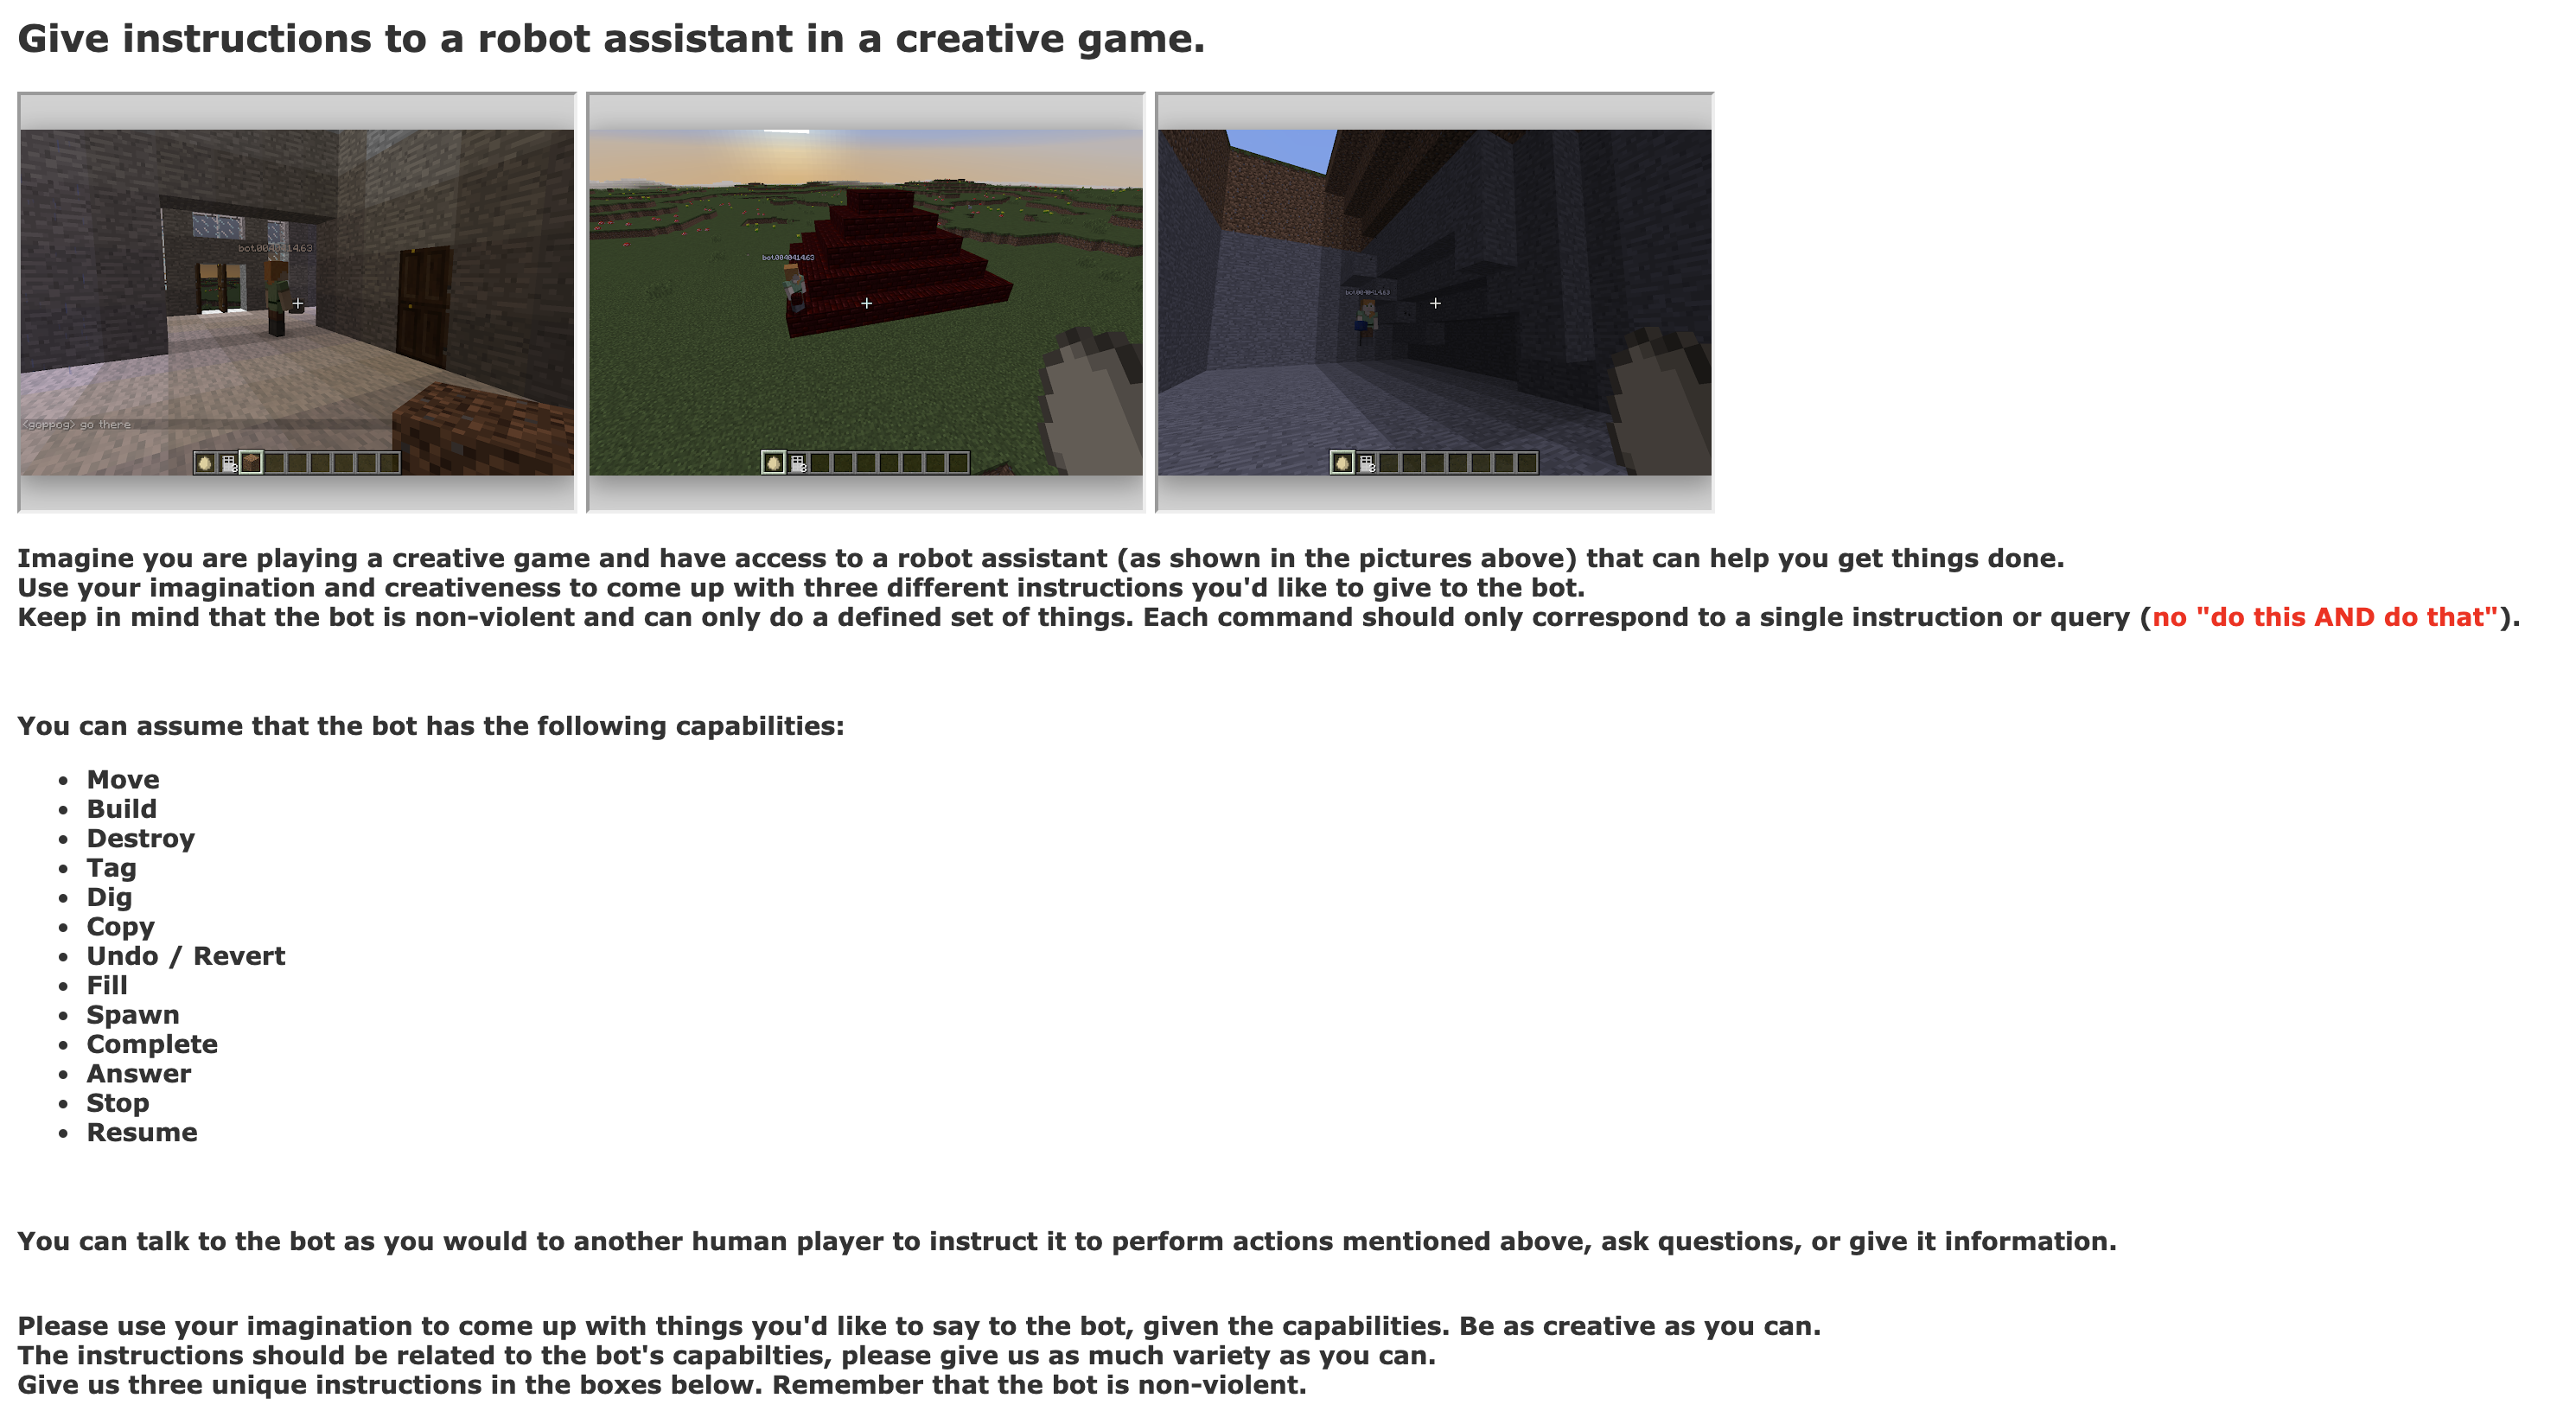
\includegraphics[width=\linewidth ]{figures/freegen.jpg}
	\caption{The task instructions shown to crowd-sourced workers for the Image and text prompts task\label{fig:freegen}}
\end{figure}

\subsection{Interactive Gameplay}
\label{sec:appen}
In this task we had crowd-sourced workers play with our bot and interact with it using in-game chat. 
The instructions shown to workers are shown in \ref{fig:appen}. 
\begin{figure}
	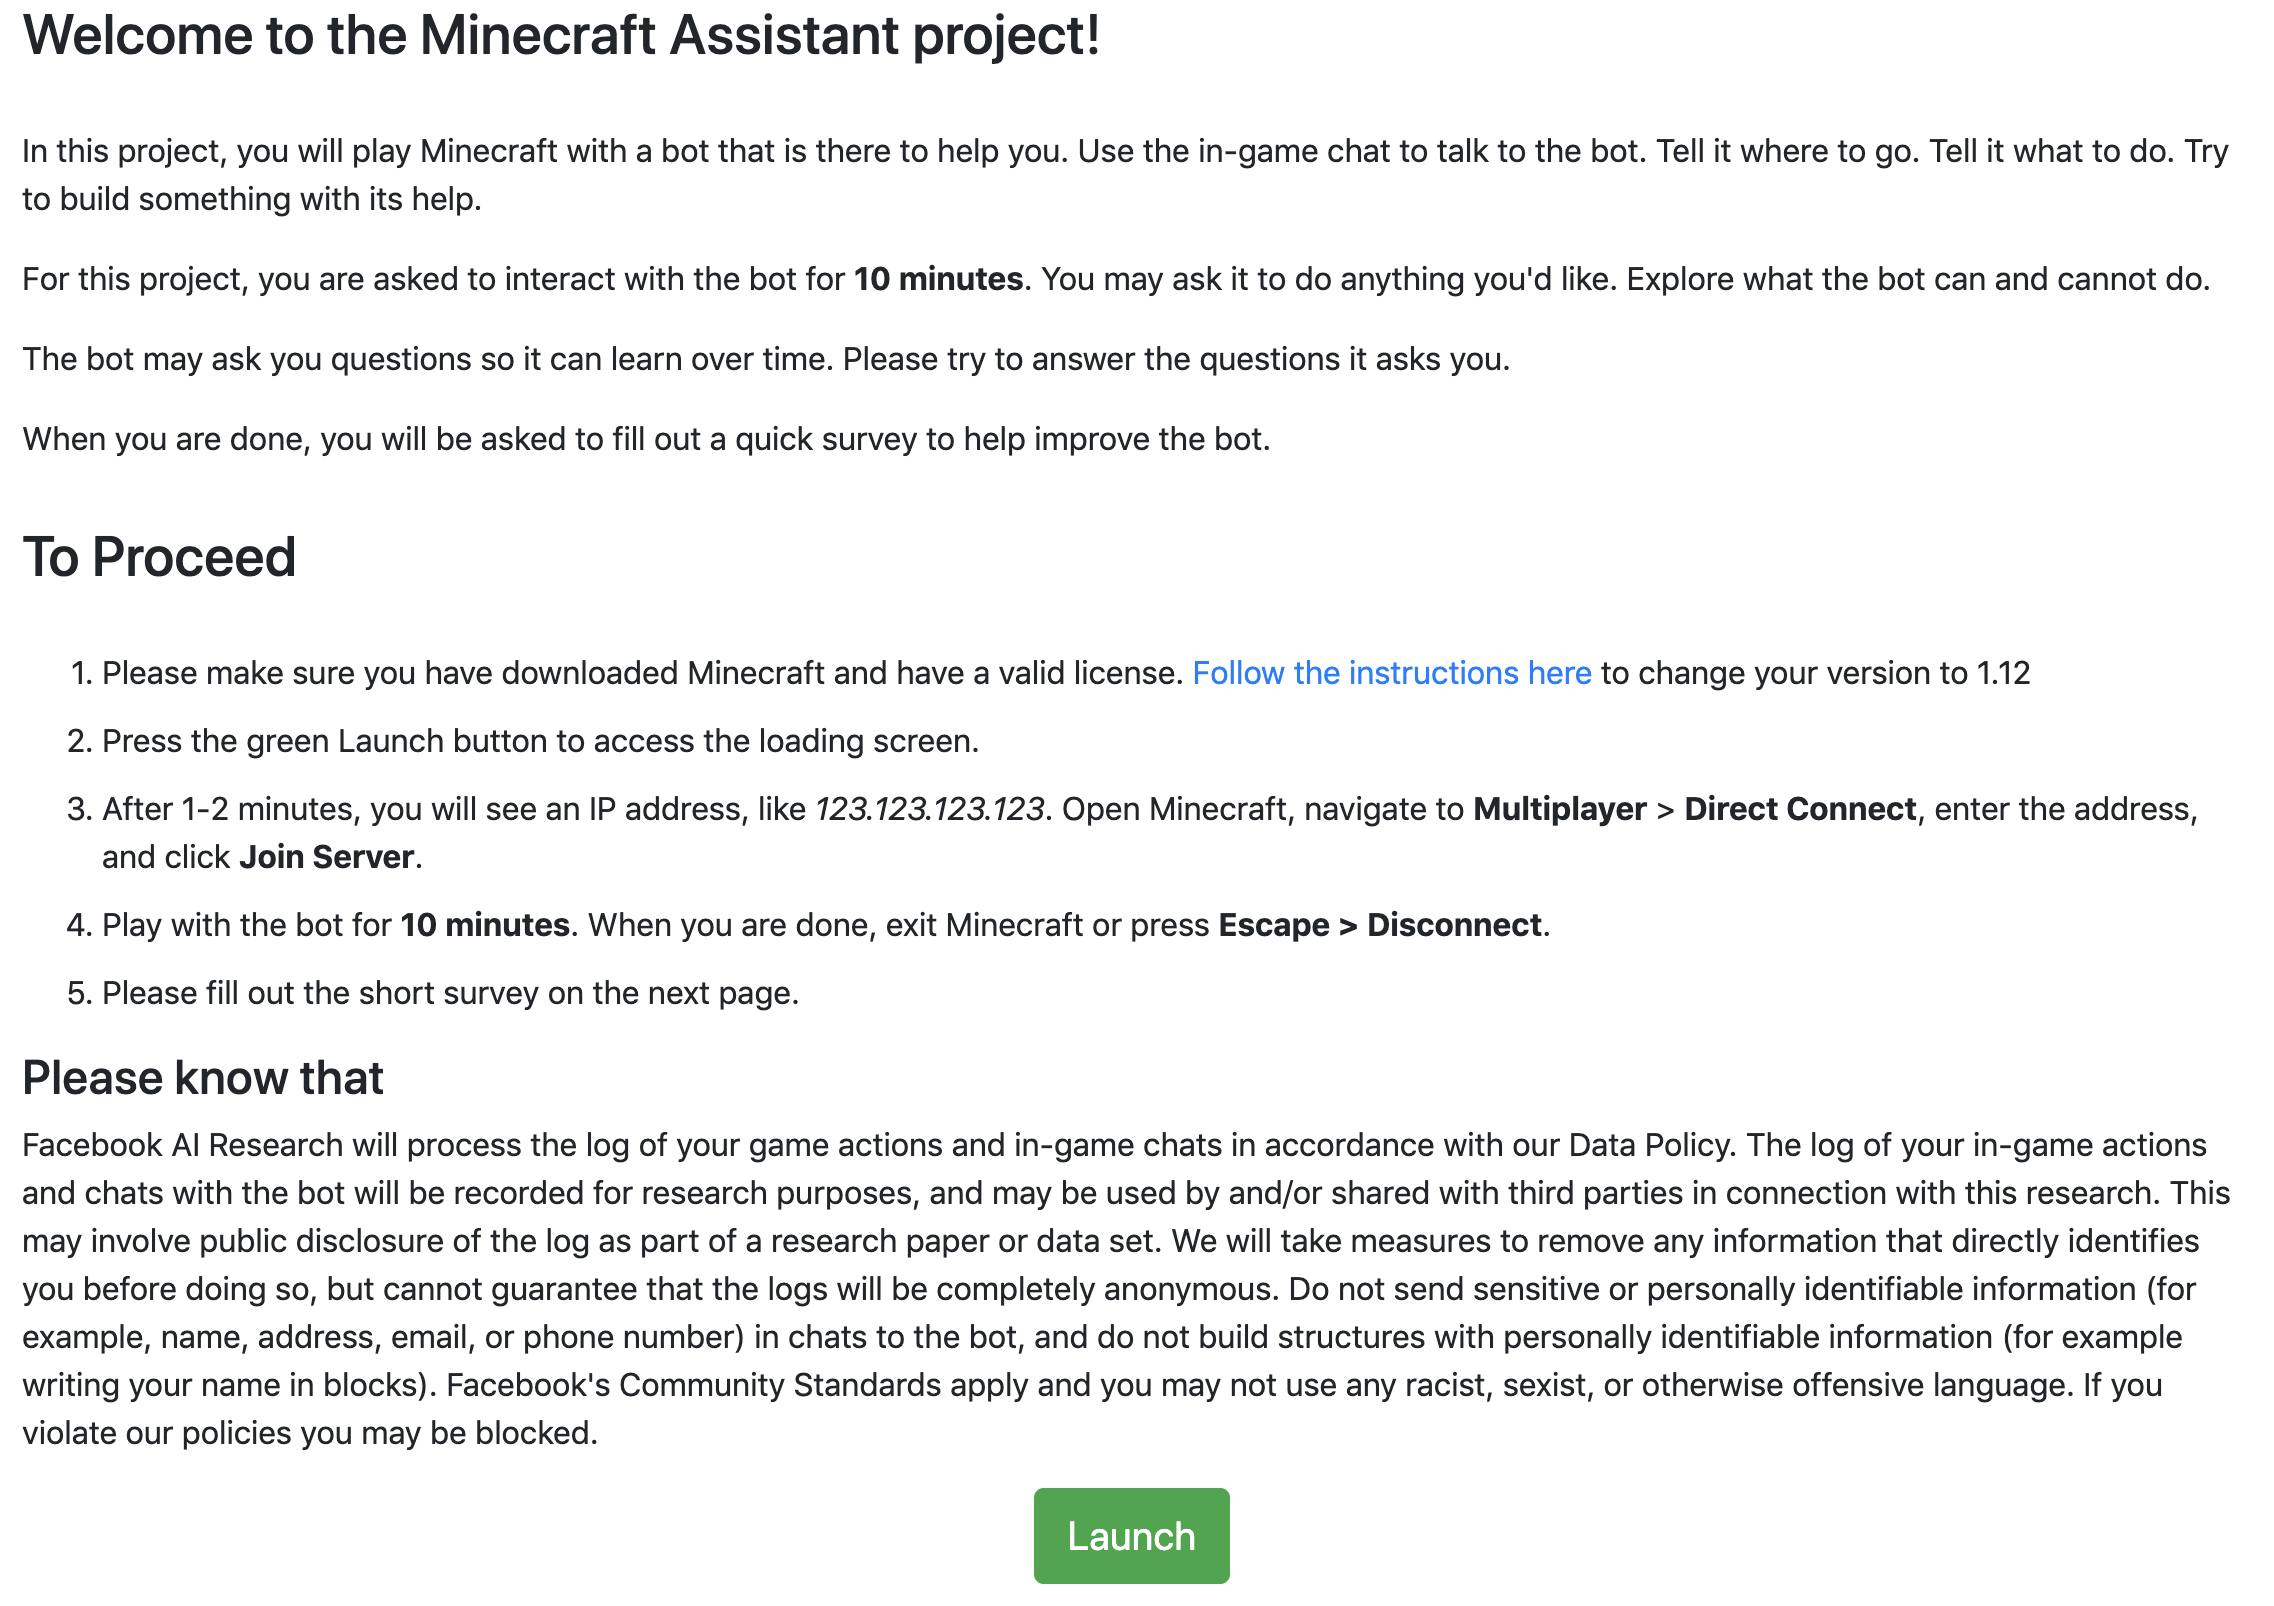
\includegraphics[width=\linewidth ]{figures/appen.png}
	\caption{The task instructions shown to crowd-sourced workers for the interactive game play\label{fig:appen}}
\end{figure}

\subsection{Annotation tool}
\label{sec:anntn}
The web based annotation tool has two subparts: Tool a and Tool b.
\subsubsection{Tool a}
This tool is the first tool in the process of annotation and asks crowd-sourced workers to help determine the intent (dialogue\_type or action\_type) of the sentence and highlight other pieces of the text based on the choices they made for the intent. (For example: if the intent was ``Build'' they are asked to select words for the thing to be built  and the location respectively.)
We also provided helpful tooltips with examples at every step of the process.

The instructions shown to workers for Tool a are shown in figure \ref{fig:annotation_task1} and step by step annotation process is shown in figure \ref{fig:annotation_step1}
\label{sec:tool_a}
\begin{figure}
	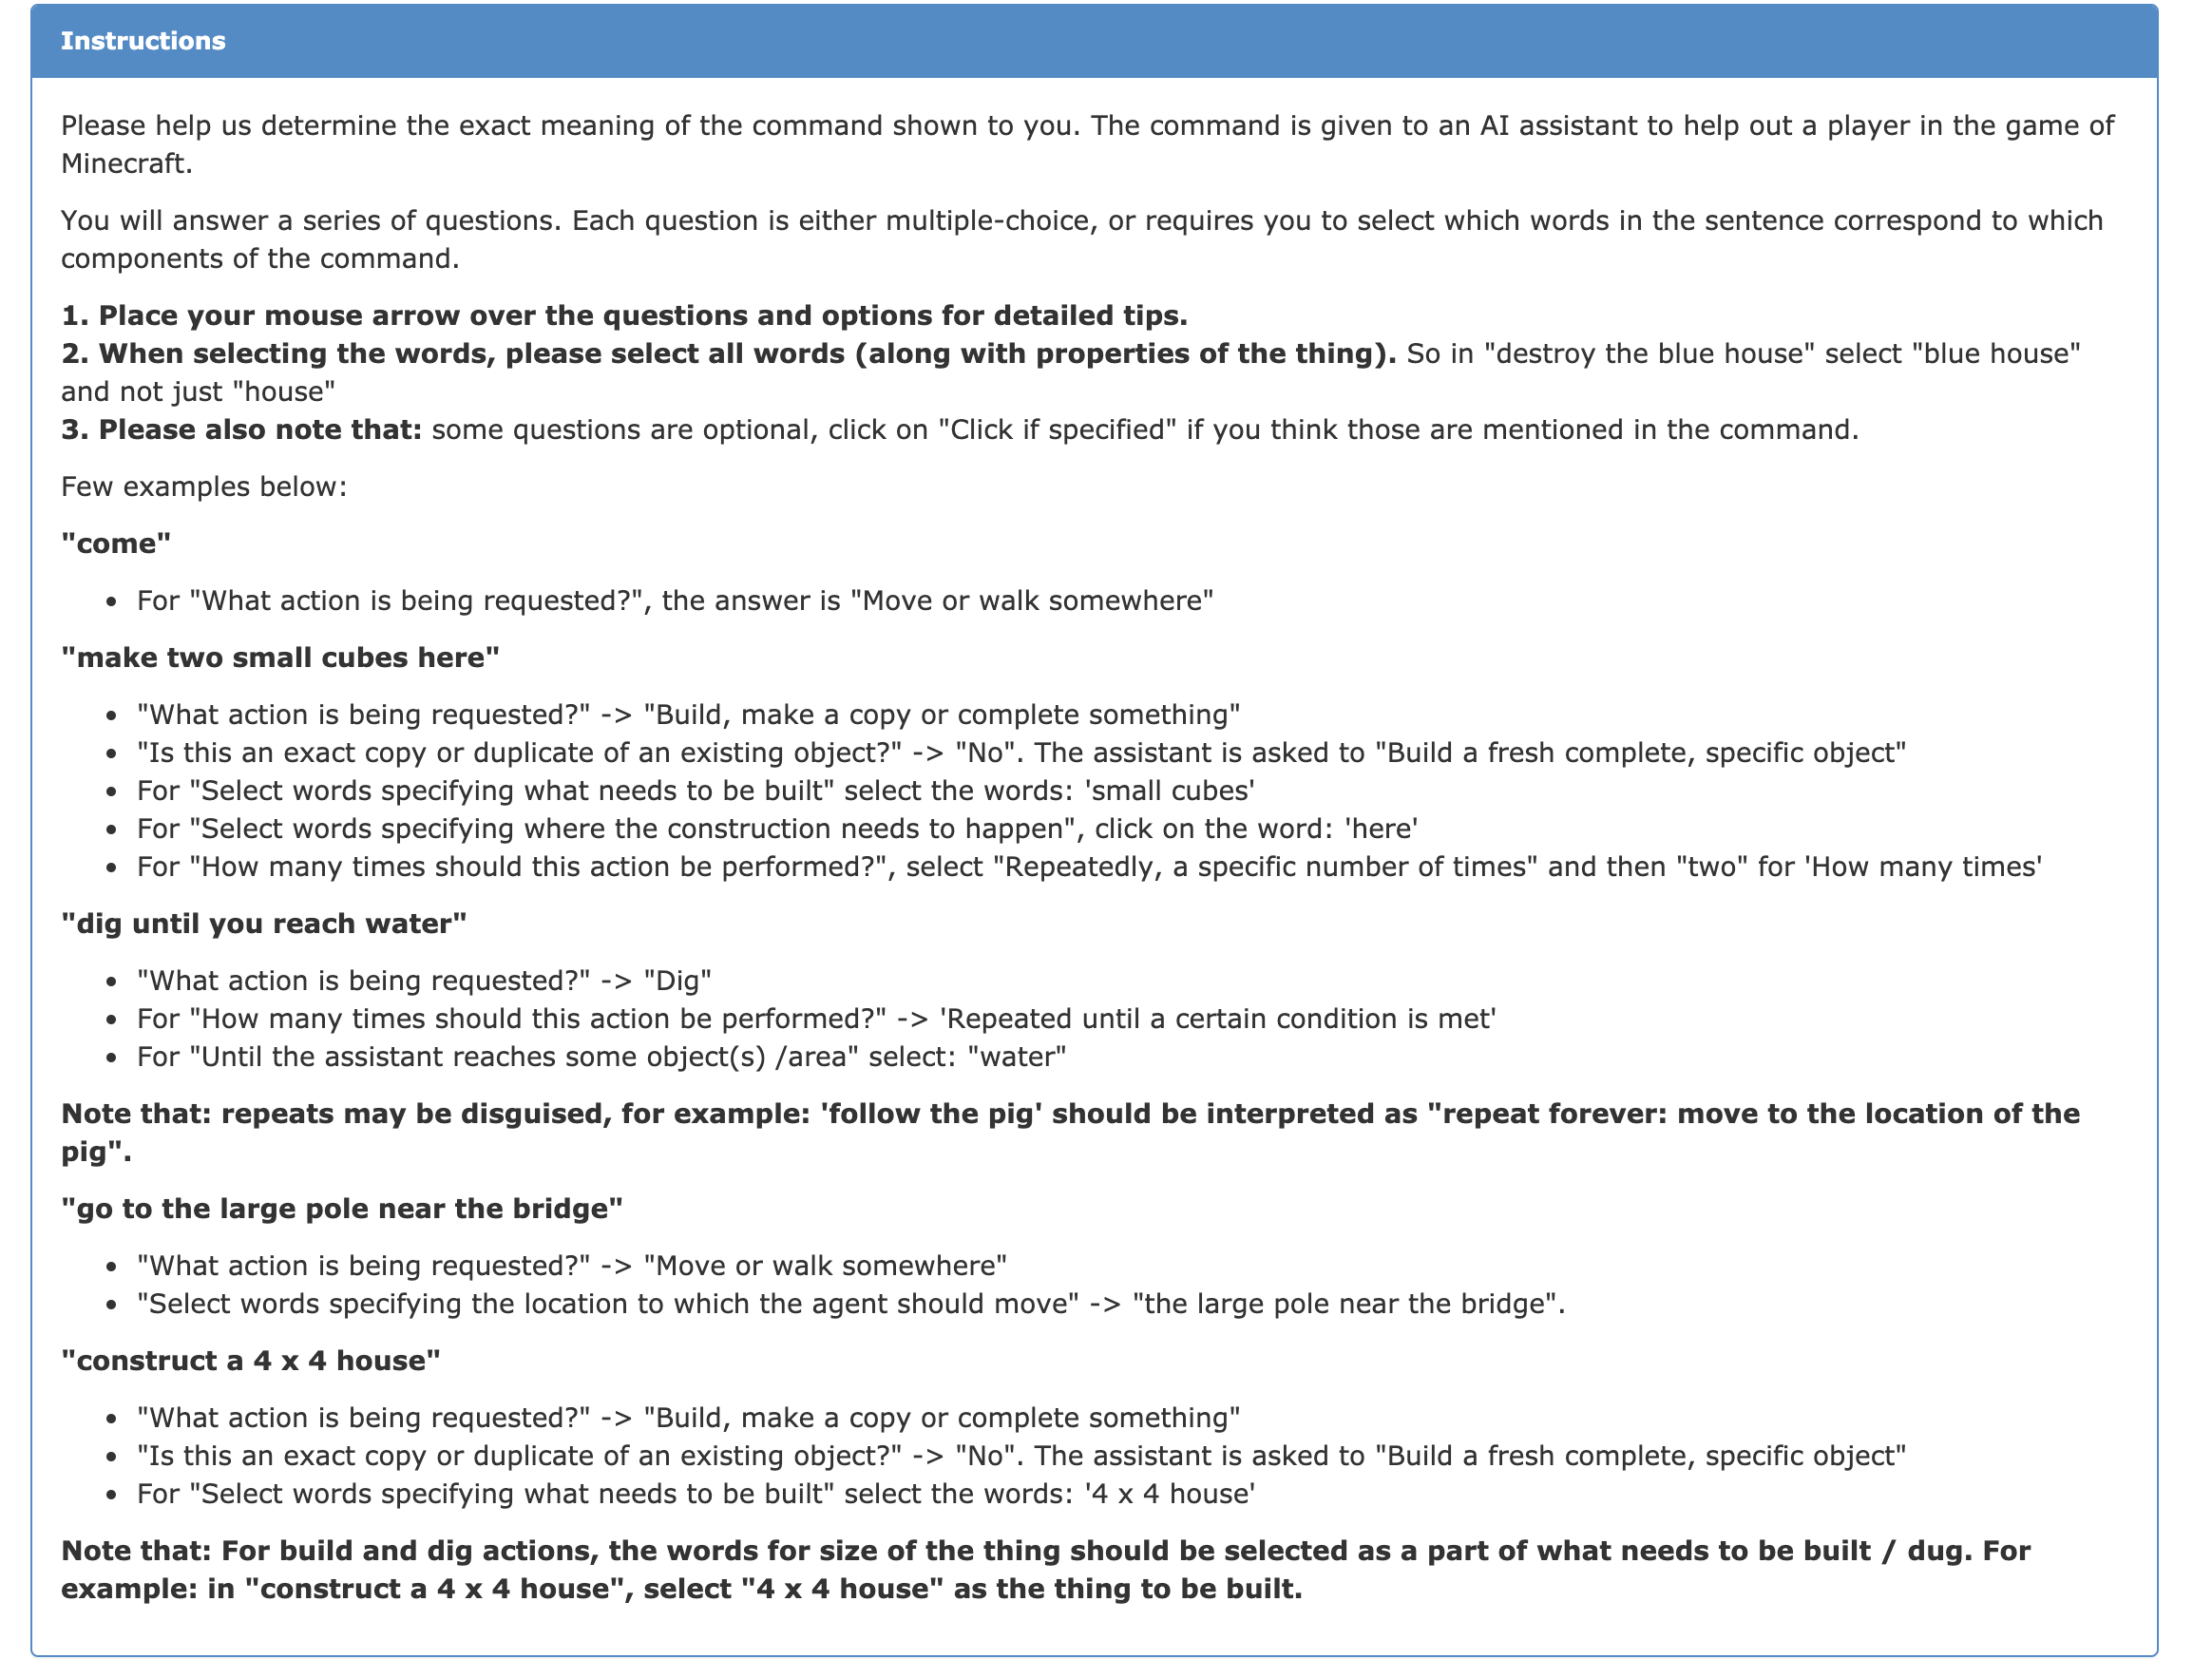
\includegraphics[width=\linewidth ]{figures/11.png}
	\caption{The task instructions shown to crowd-sourced workers for the annotation Tool a}
	\label{fig:annotation_task1}
\end{figure}

\begin{figure}[h]

    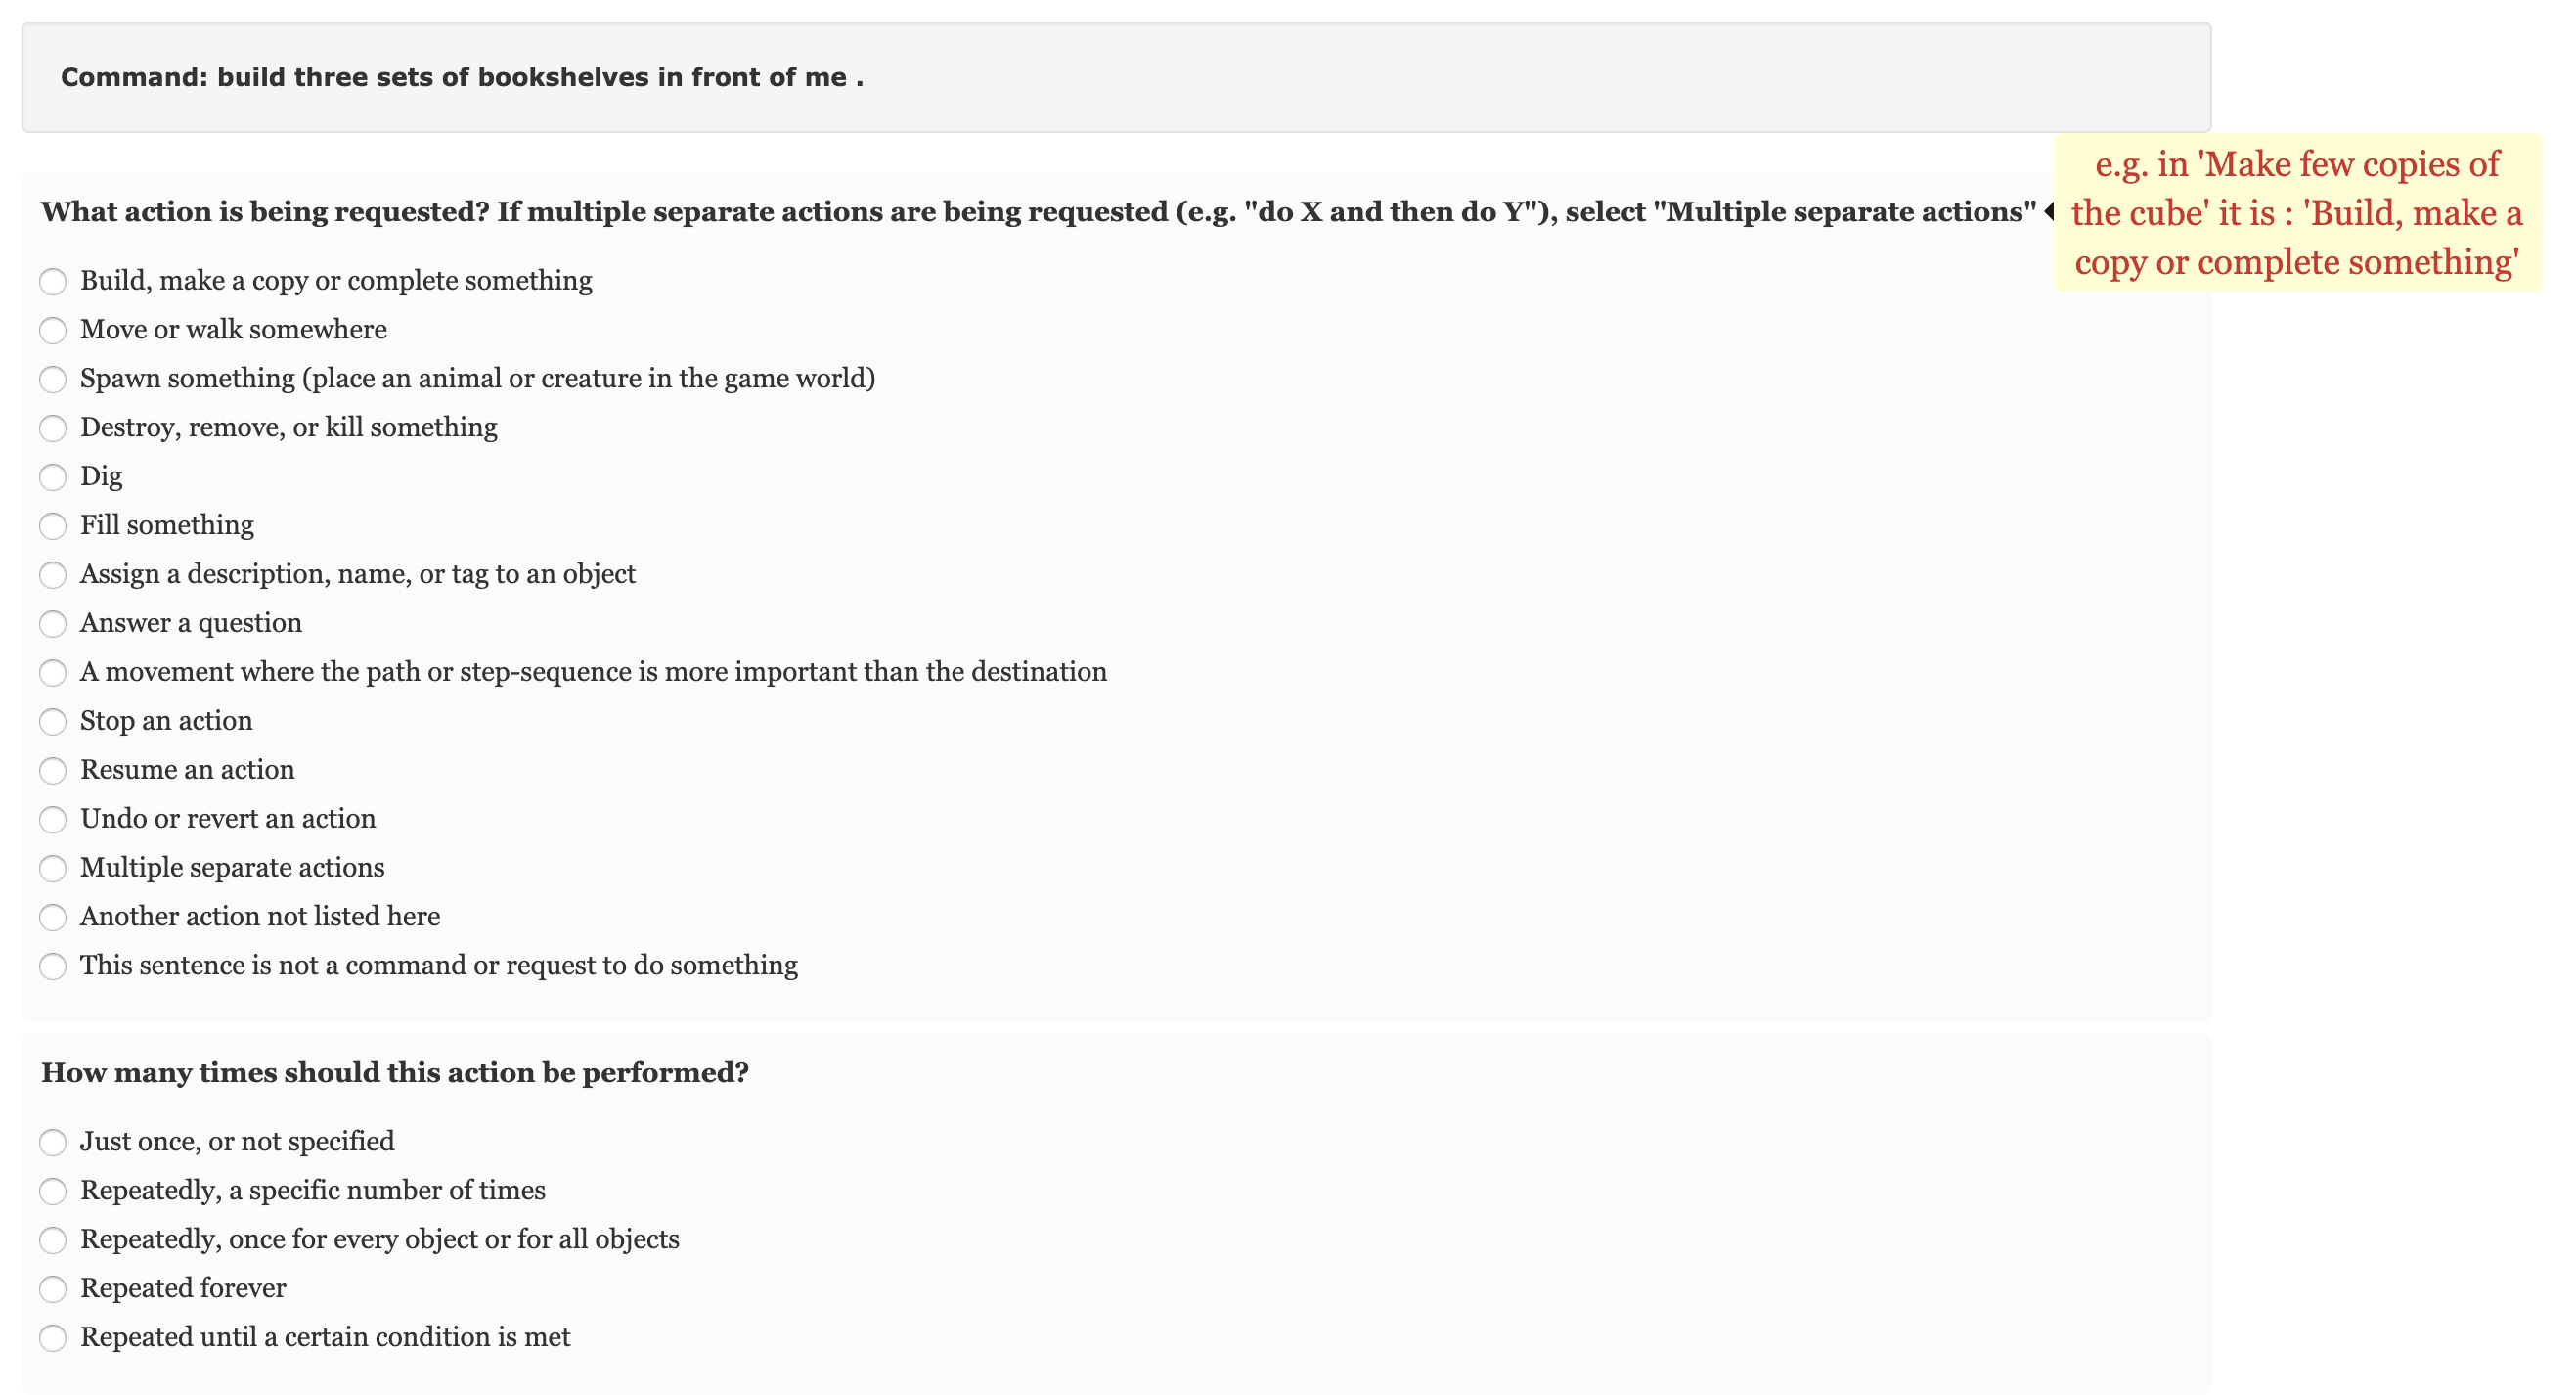
\includegraphics[width=\linewidth, height=6cm, ,keepaspectratio  ]{figures/12.png}
    \bigbreak
     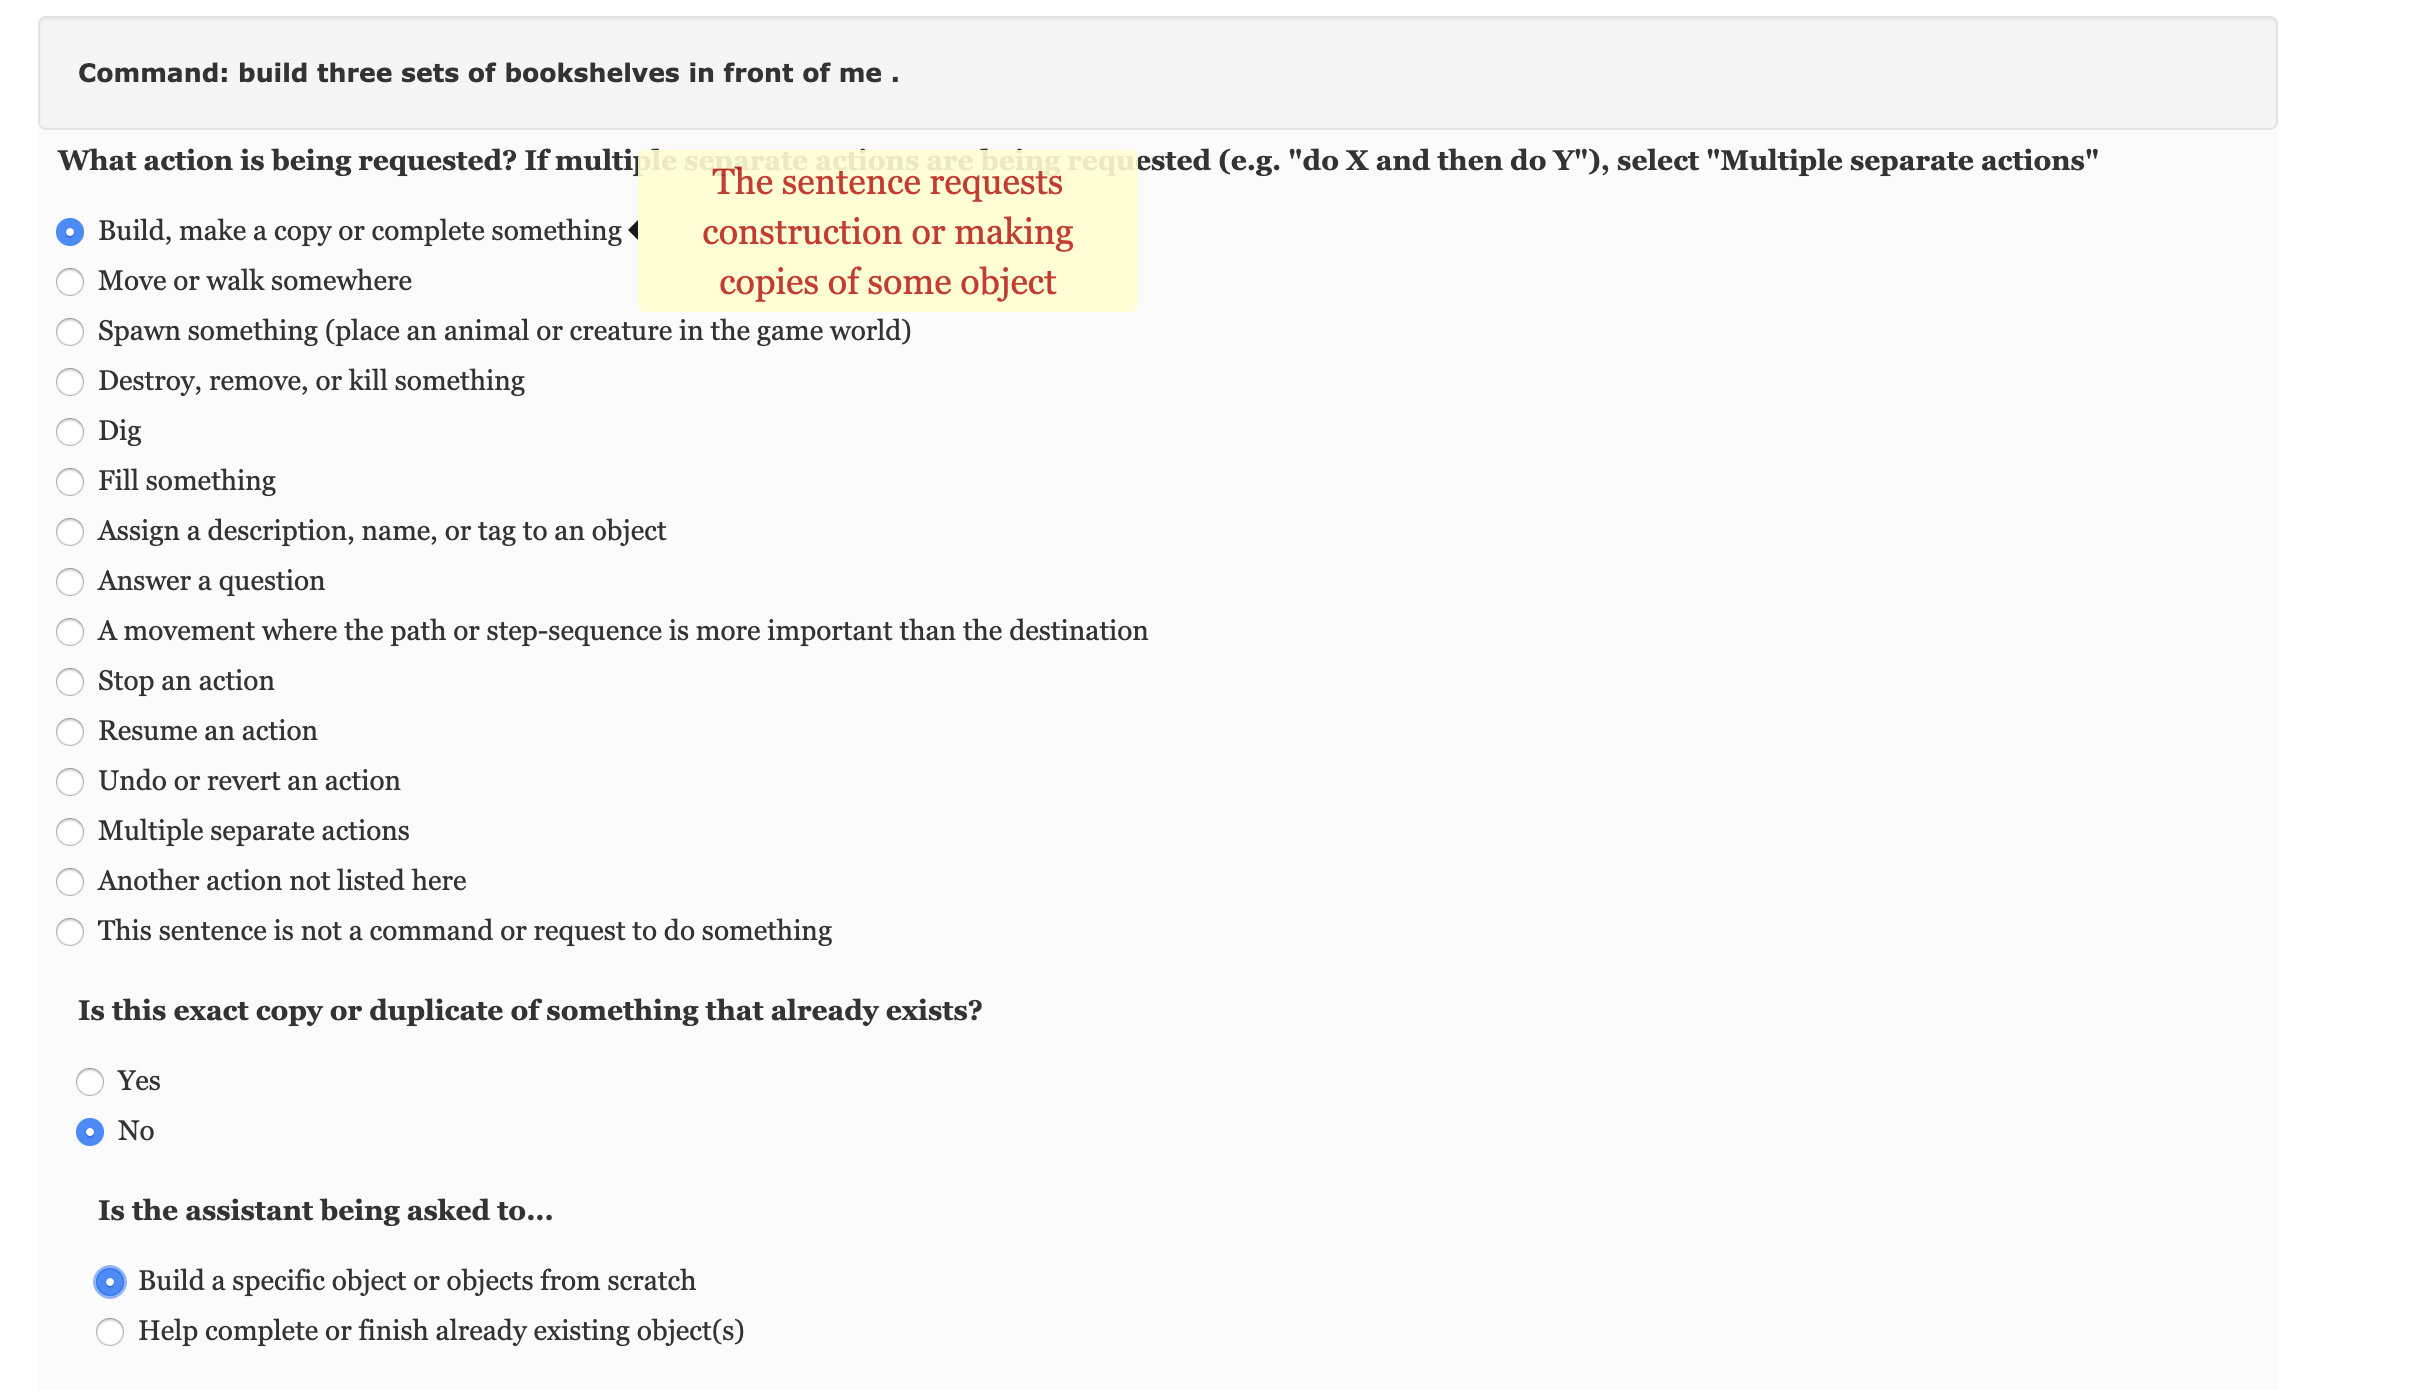
\includegraphics[width=\linewidth, height=6cm, ,keepaspectratio  ]{figures/13.png} 
     \bigbreak
     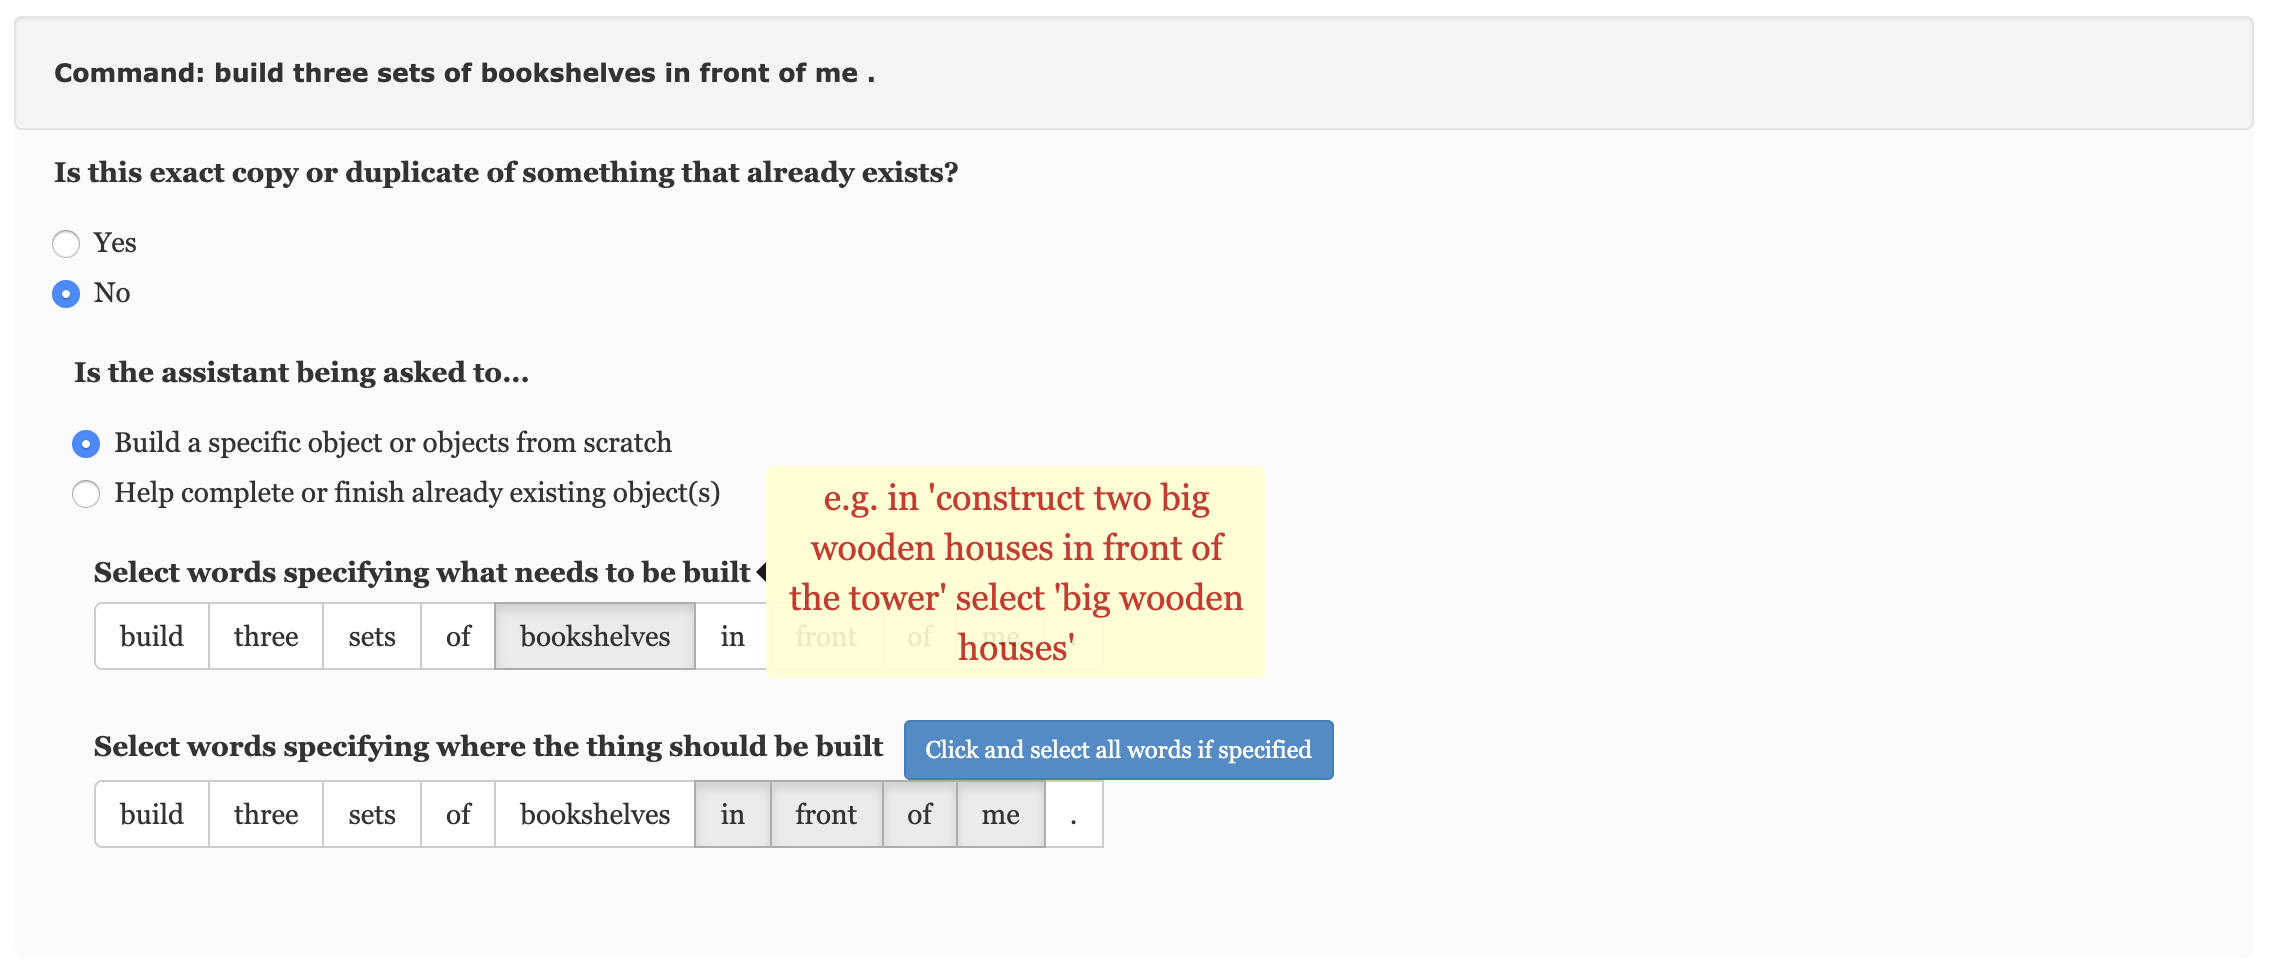
\includegraphics[width=0.65\linewidth, height=6cm, ,keepaspectratio ]{figures/14.png}
     \bigbreak
     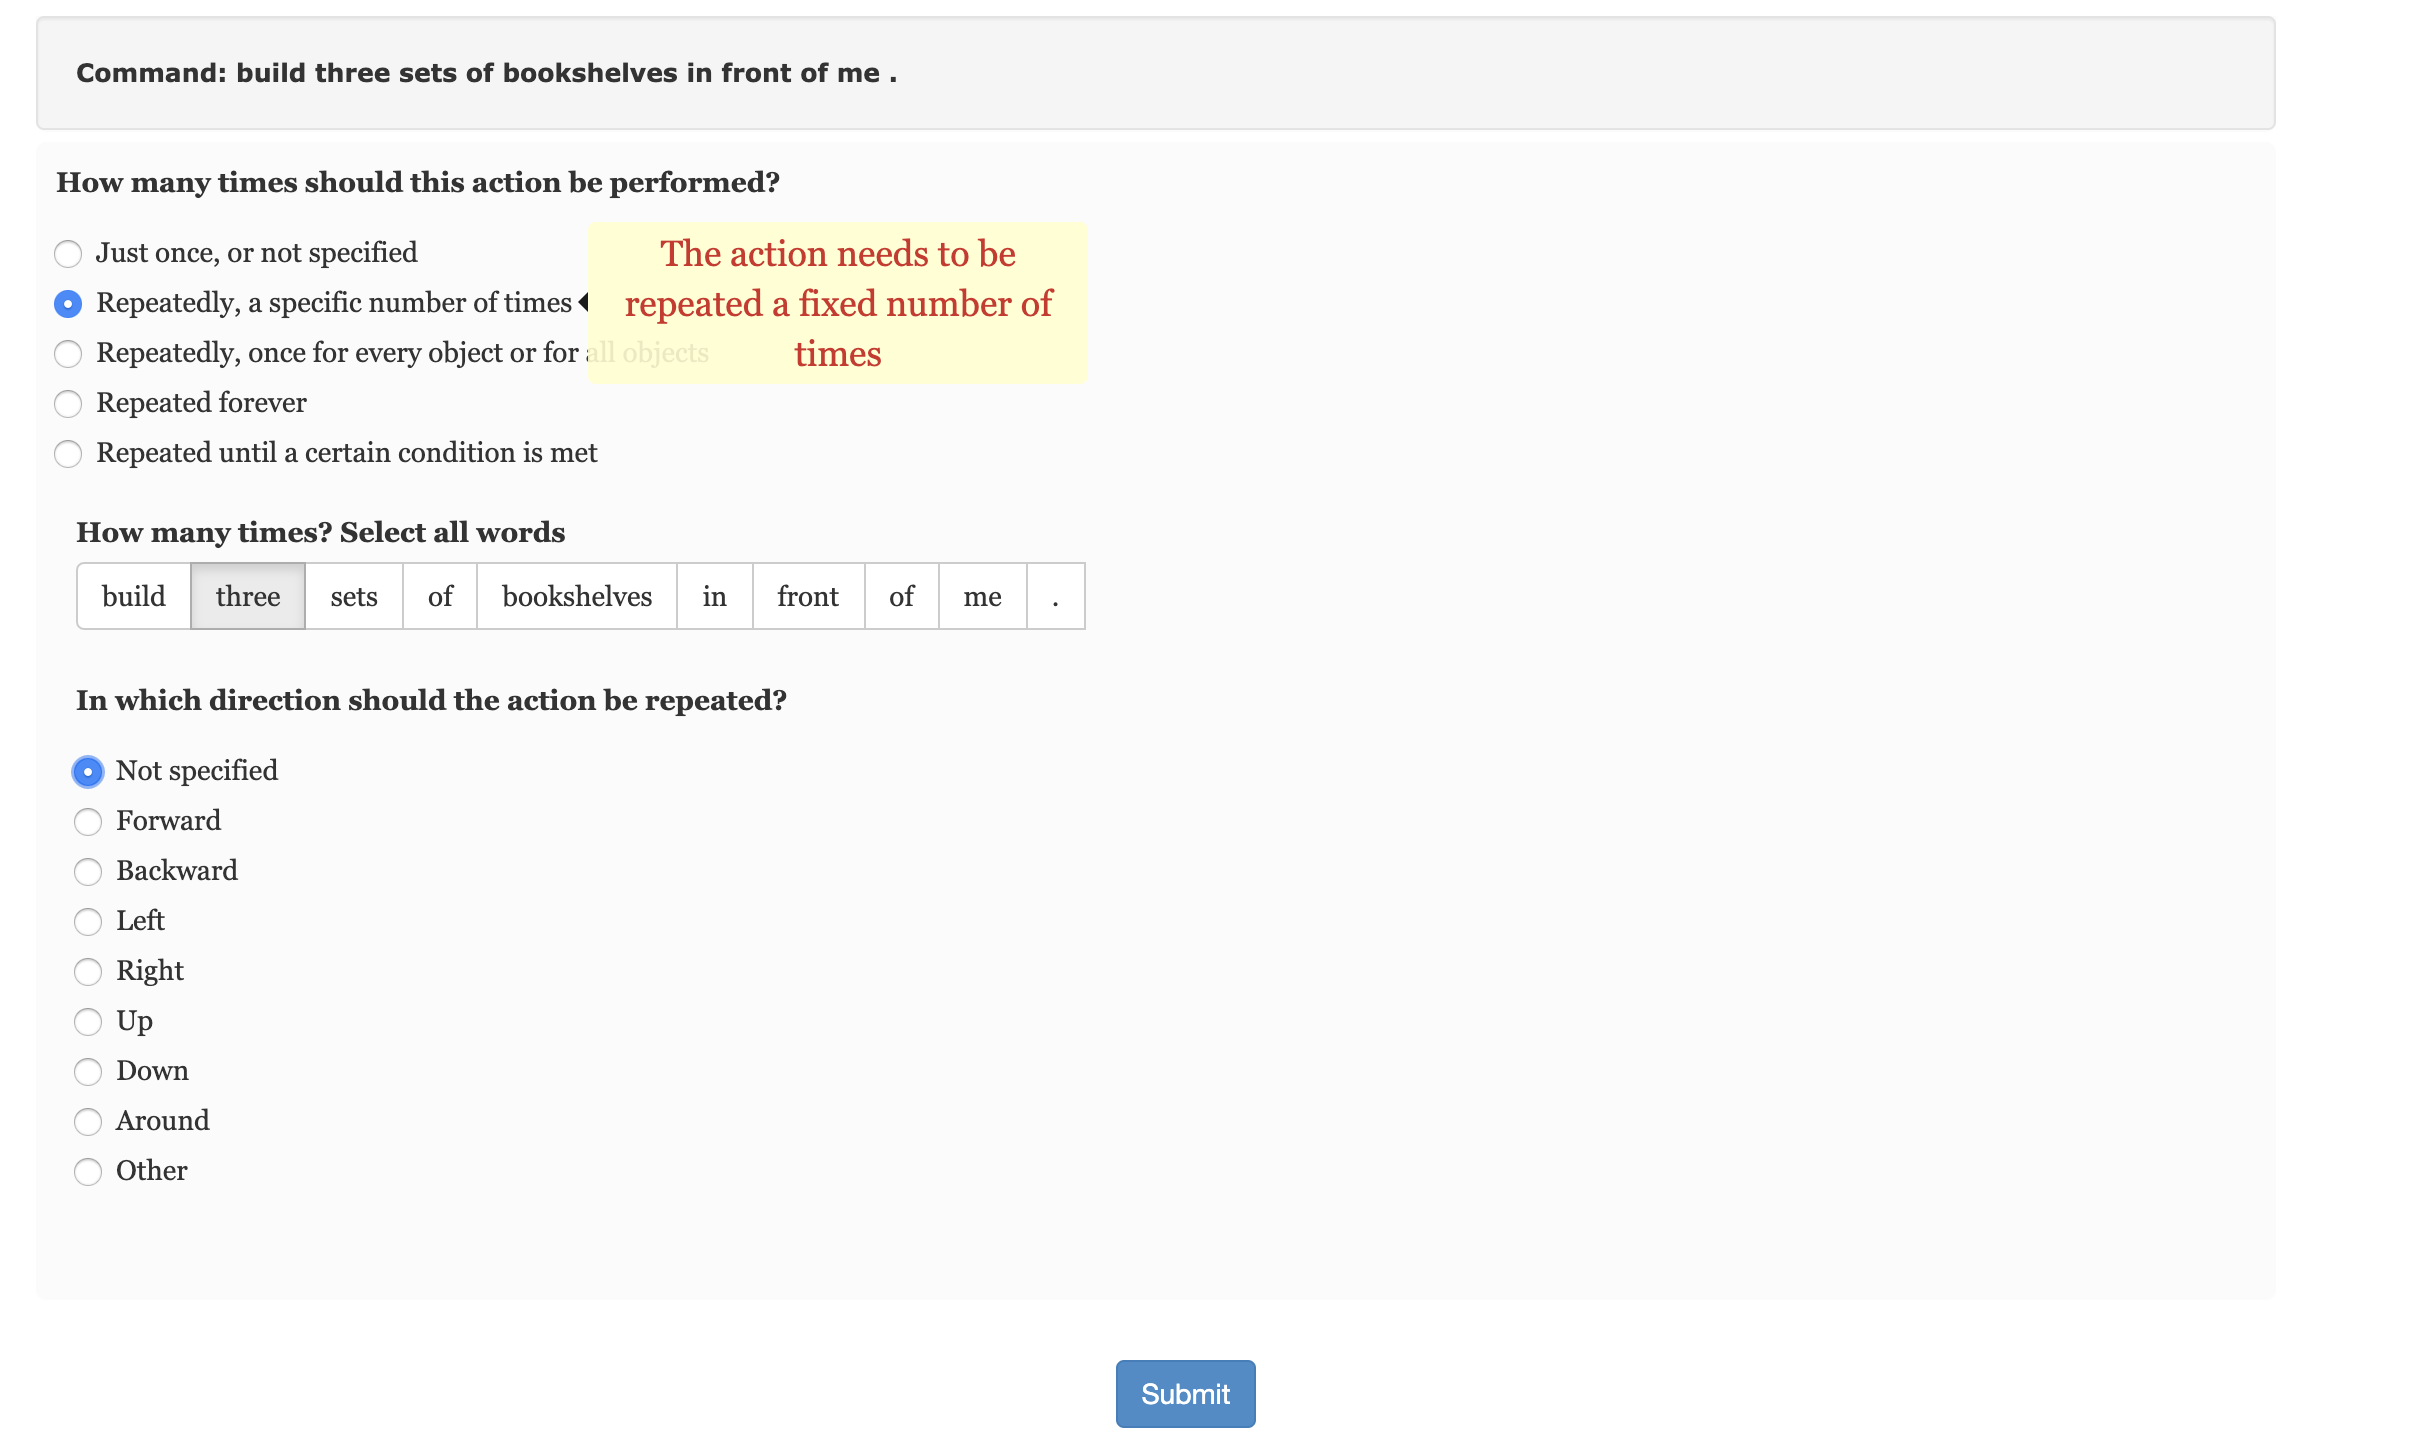
\includegraphics[width=\linewidth, height=6cm, ,keepaspectratio]{figures/15.png}
	 \caption{The step by step screenshot of annotations process for the command: ``build three sets of bookshelves in front of me .''  in Tool a}
	\label{fig:annotation_step1}
\end{figure}

\subsubsection{Tool b}
After we determine the intent from Tool a and get highlighted span of words for respective children of the intent, we use this tool.
This is the second tool in the annotation process and asks crowd-sourced workers to help determine the fin-grained properties of specific entities of the action or dialogue. Note that we already got the words representing these, highlighted in \ref{sec:tool_a}. For example : the words `` big bright house'' are highlighted in the sentence ``destroy the big bright house by the tree '' as an outcome of Tool a.
The questionnaire changes dynamically based on the choices the workers make at every step of the tool. We provided helpful tooltips with examples at every step of the annotation process.
Using the output of Tool a and Tool b, we can successfully construct the entire logical form for a given sentence.

The instructions shown to workers for Tool b are shown in Figure \ref{fig:annotation_task2} and step by step annotation process for annotating properties of ``location'' in a ``Move'' action is shown in Figure \ref{fig:move_location} and annotating ``reference\_object'' in ``Destroy'' action is shown in Figure \ref{fig:destroy_ref}
 

\label{sec:tool_b}

\begin{figure}
	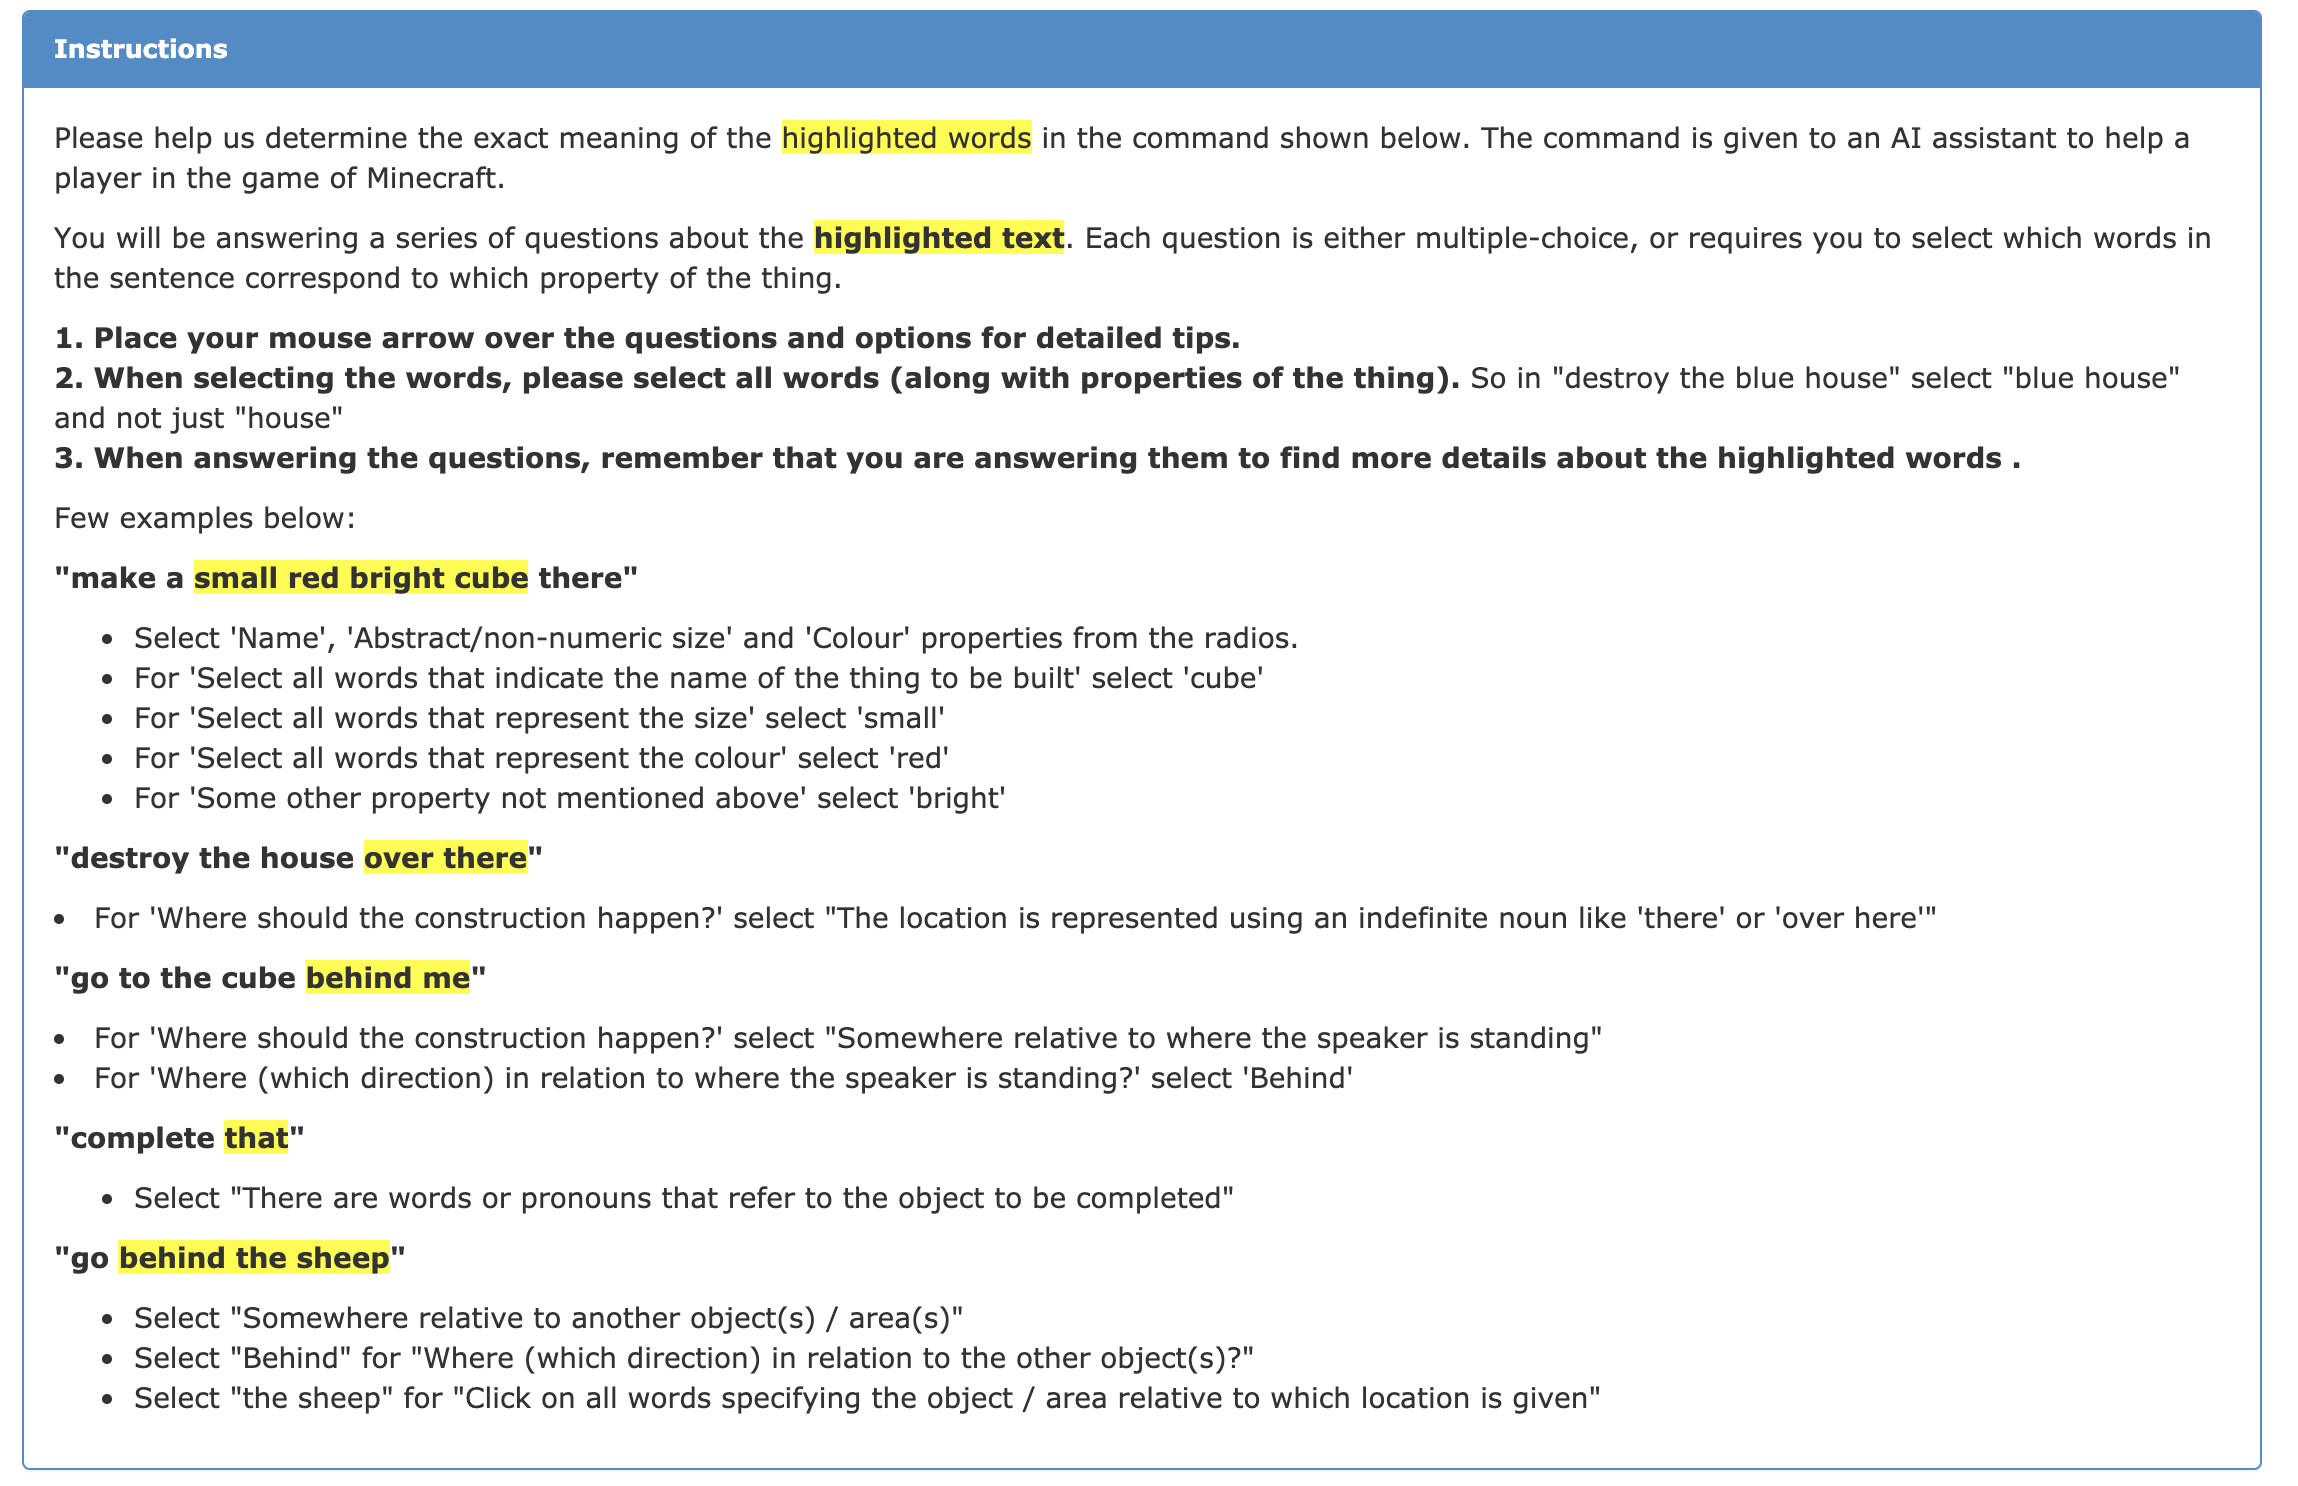
\includegraphics[width=\linewidth ]{figures/21.png}
	\caption{The task instructions shown to crowd-sourced workers for the annotation Tool b}
	\label{fig:annotation_task2}
\end{figure}

\begin{figure}[h]
    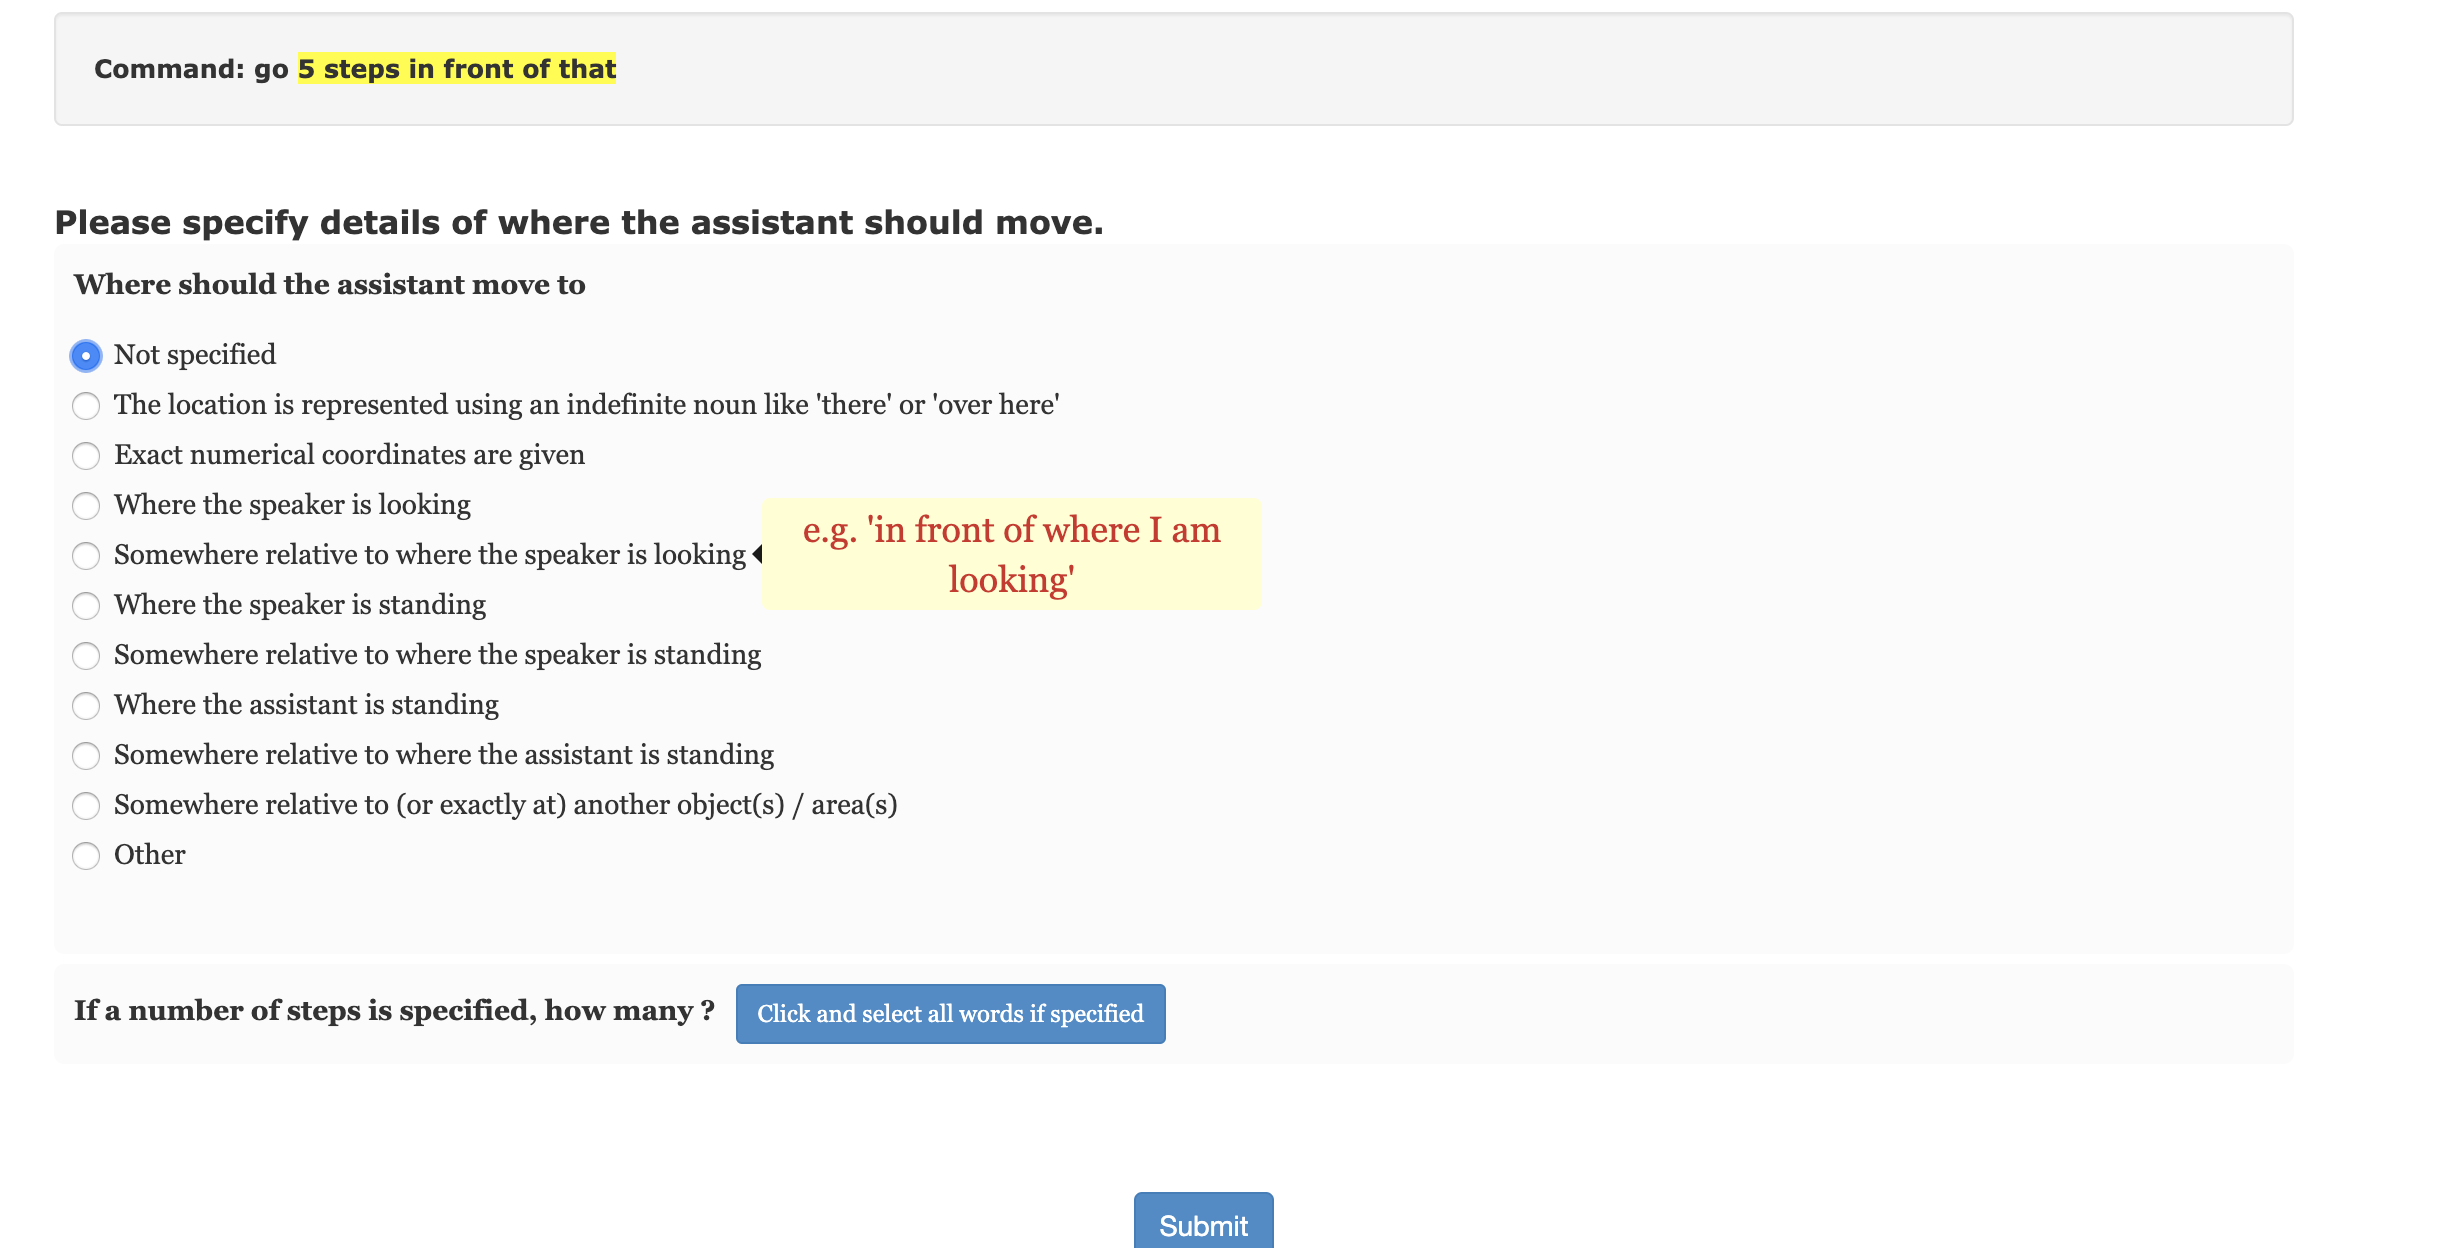
\includegraphics[width=\linewidth, height=6cm, ,keepaspectratio  ]{figures/22.png}
    \bigbreak
     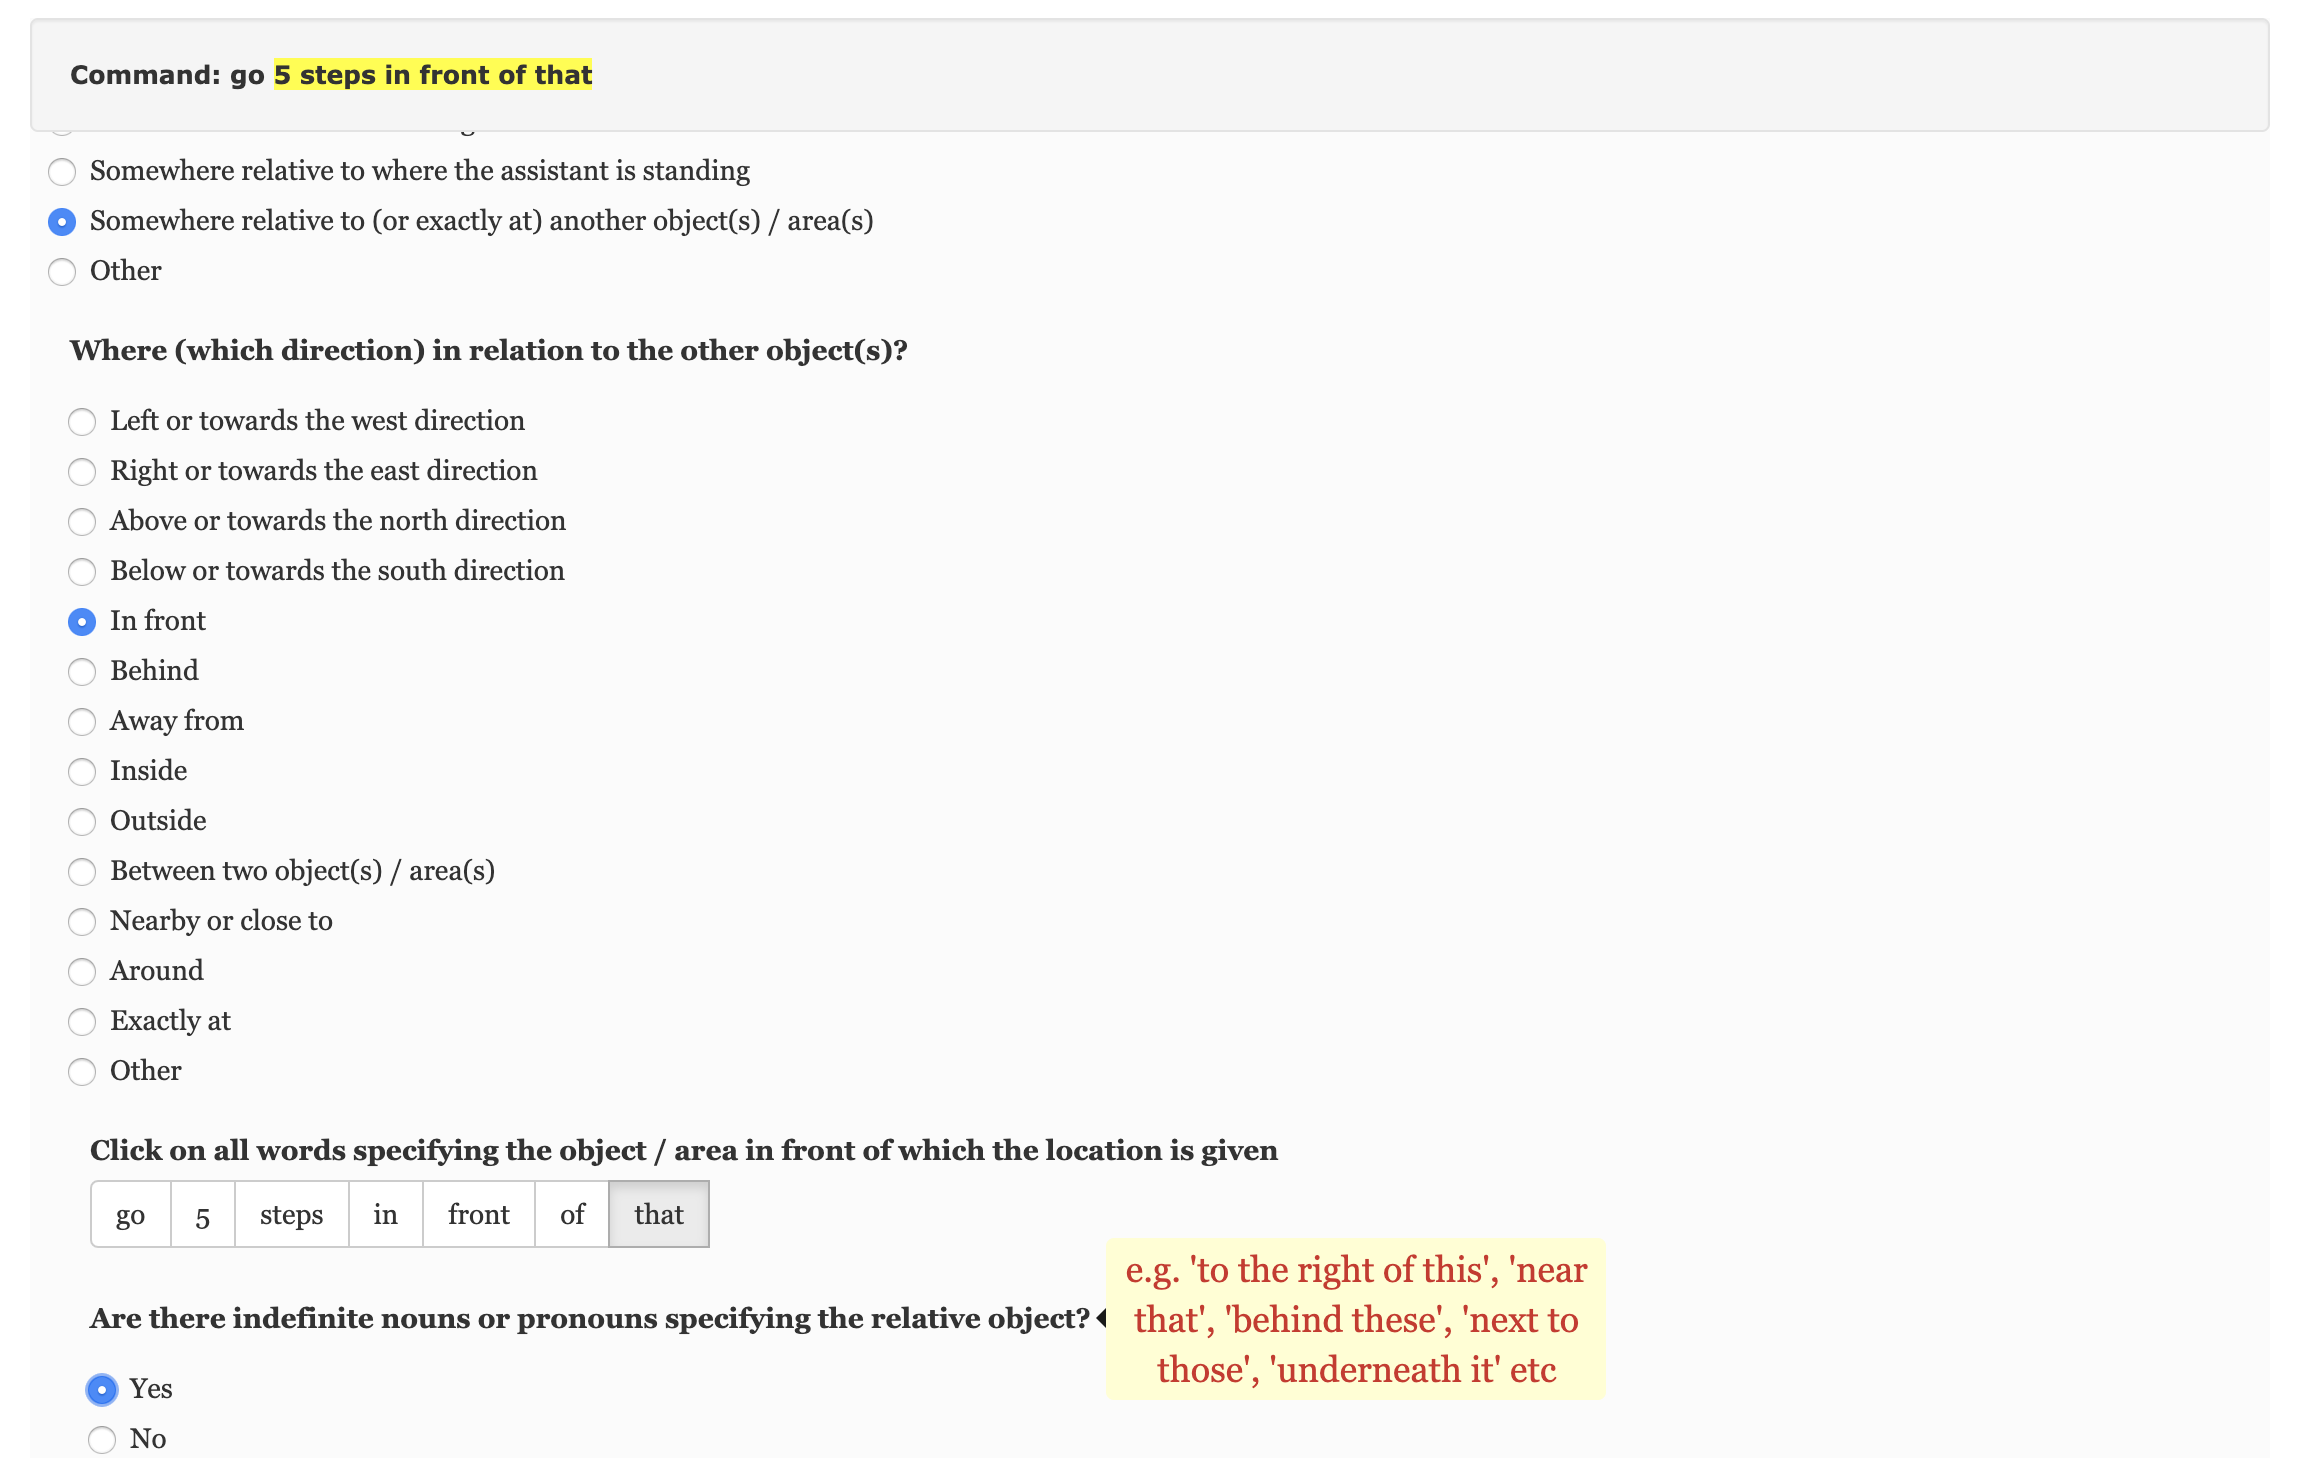
\includegraphics[width=\linewidth, height=6cm, ,keepaspectratio  ]{figures/23.png} 
     \bigbreak
     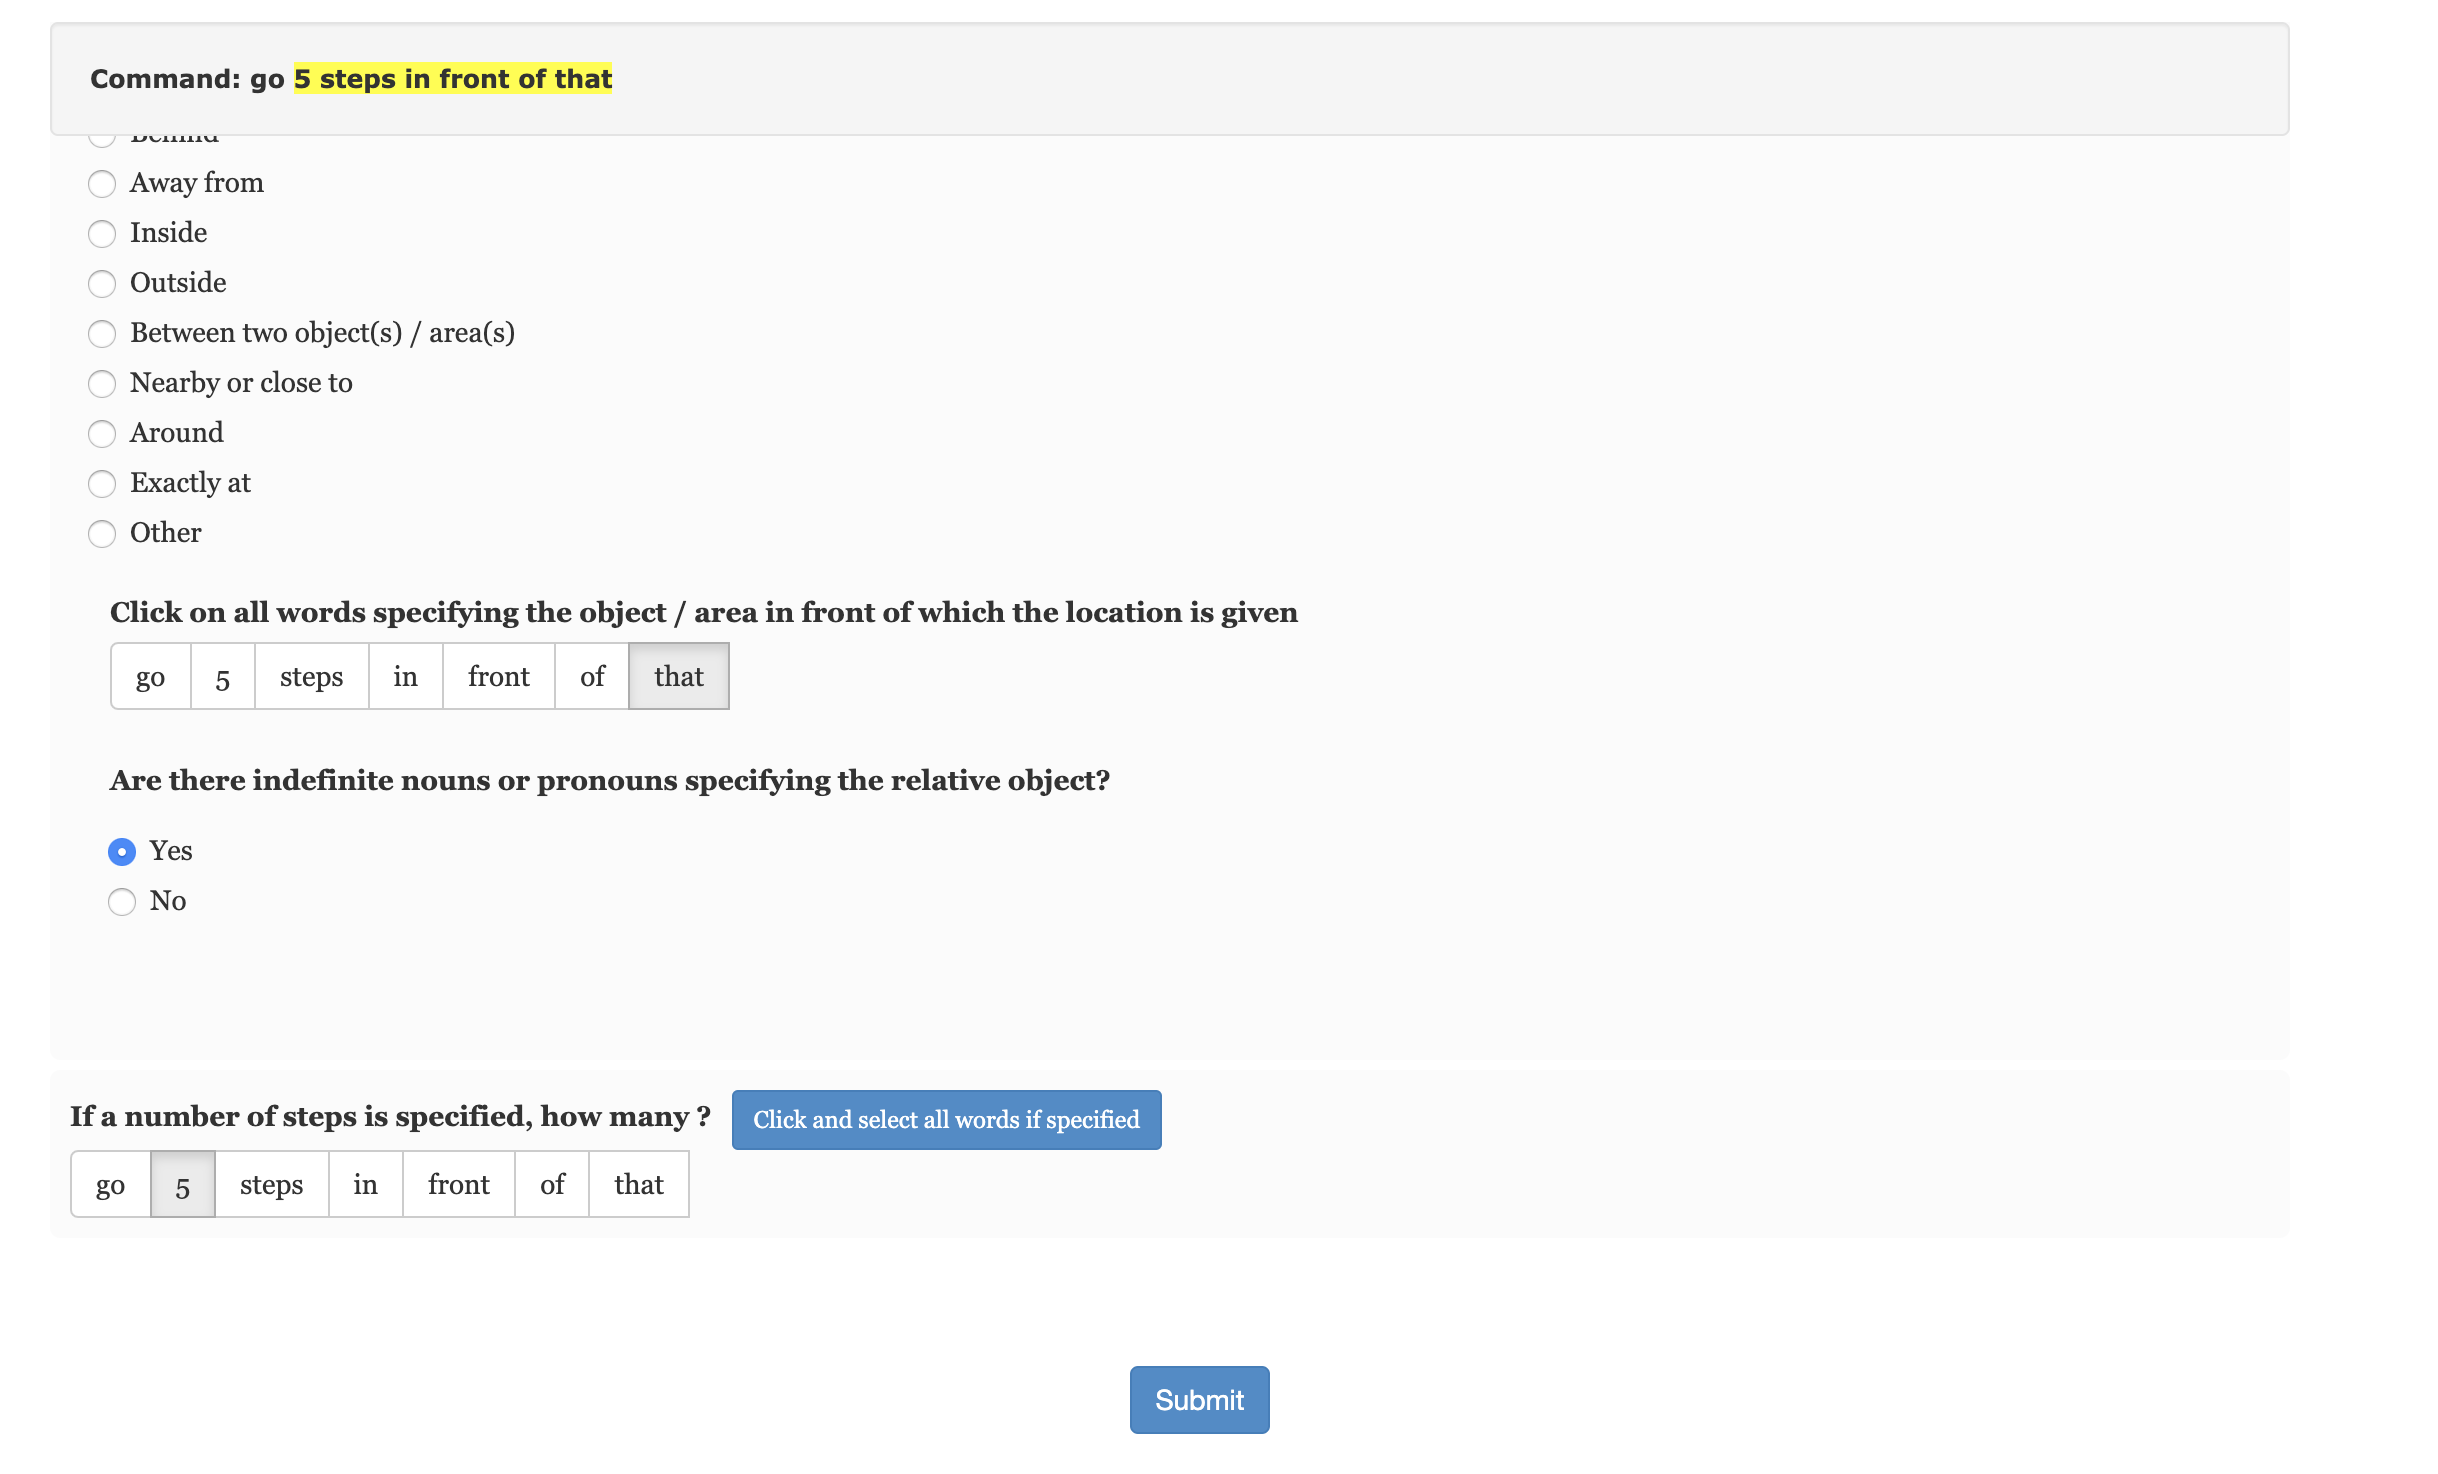
\includegraphics[width=0.65\linewidth, height=6cm, keepaspectratio ]{figures/24.png}
	 \caption{The step by step screenshot of annotating properties of highlighted words for``location''  in a ``Move'' action.}
	\label{fig:move_location}
\end{figure}

\begin{figure}[h]
    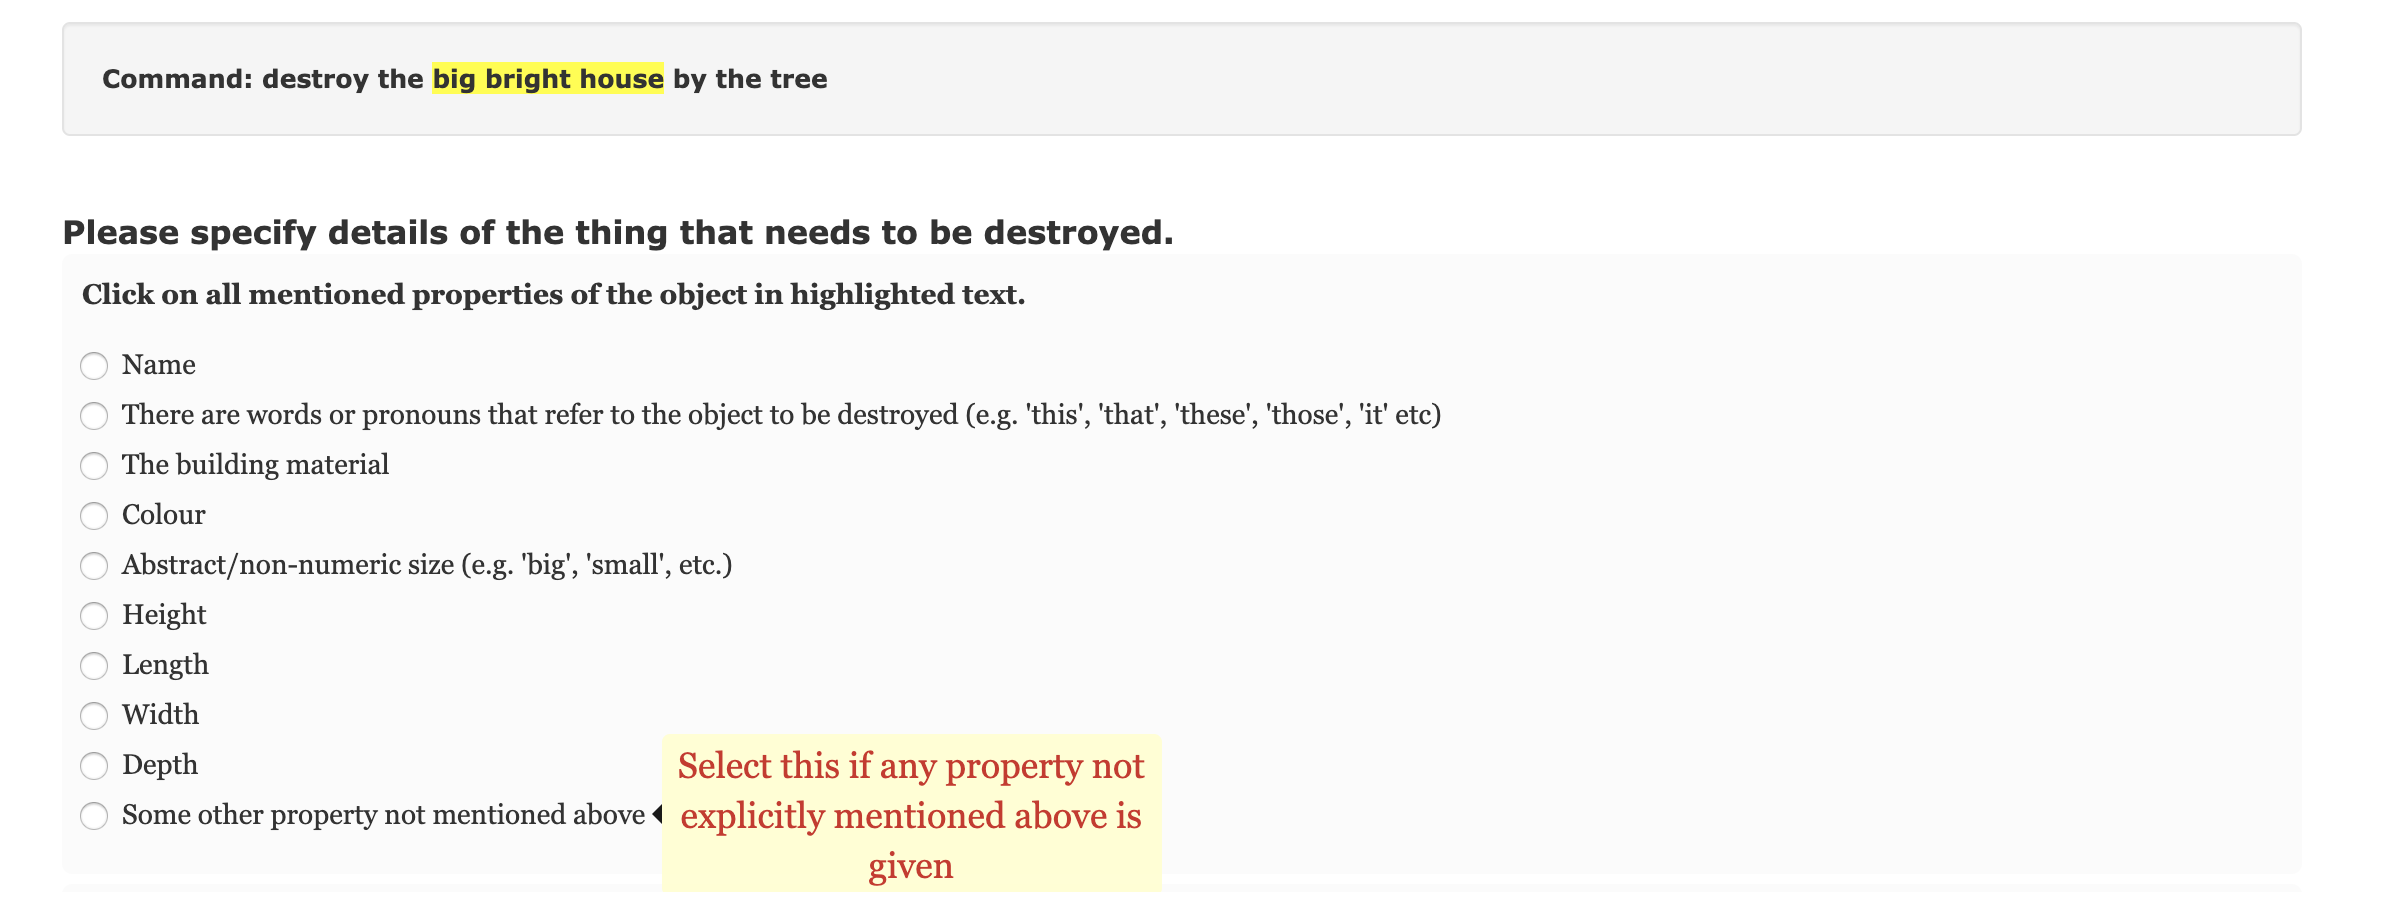
\includegraphics[width=0.70\linewidth, height=6cm, ,keepaspectratio  ]{figures/25.png}
    \bigbreak
     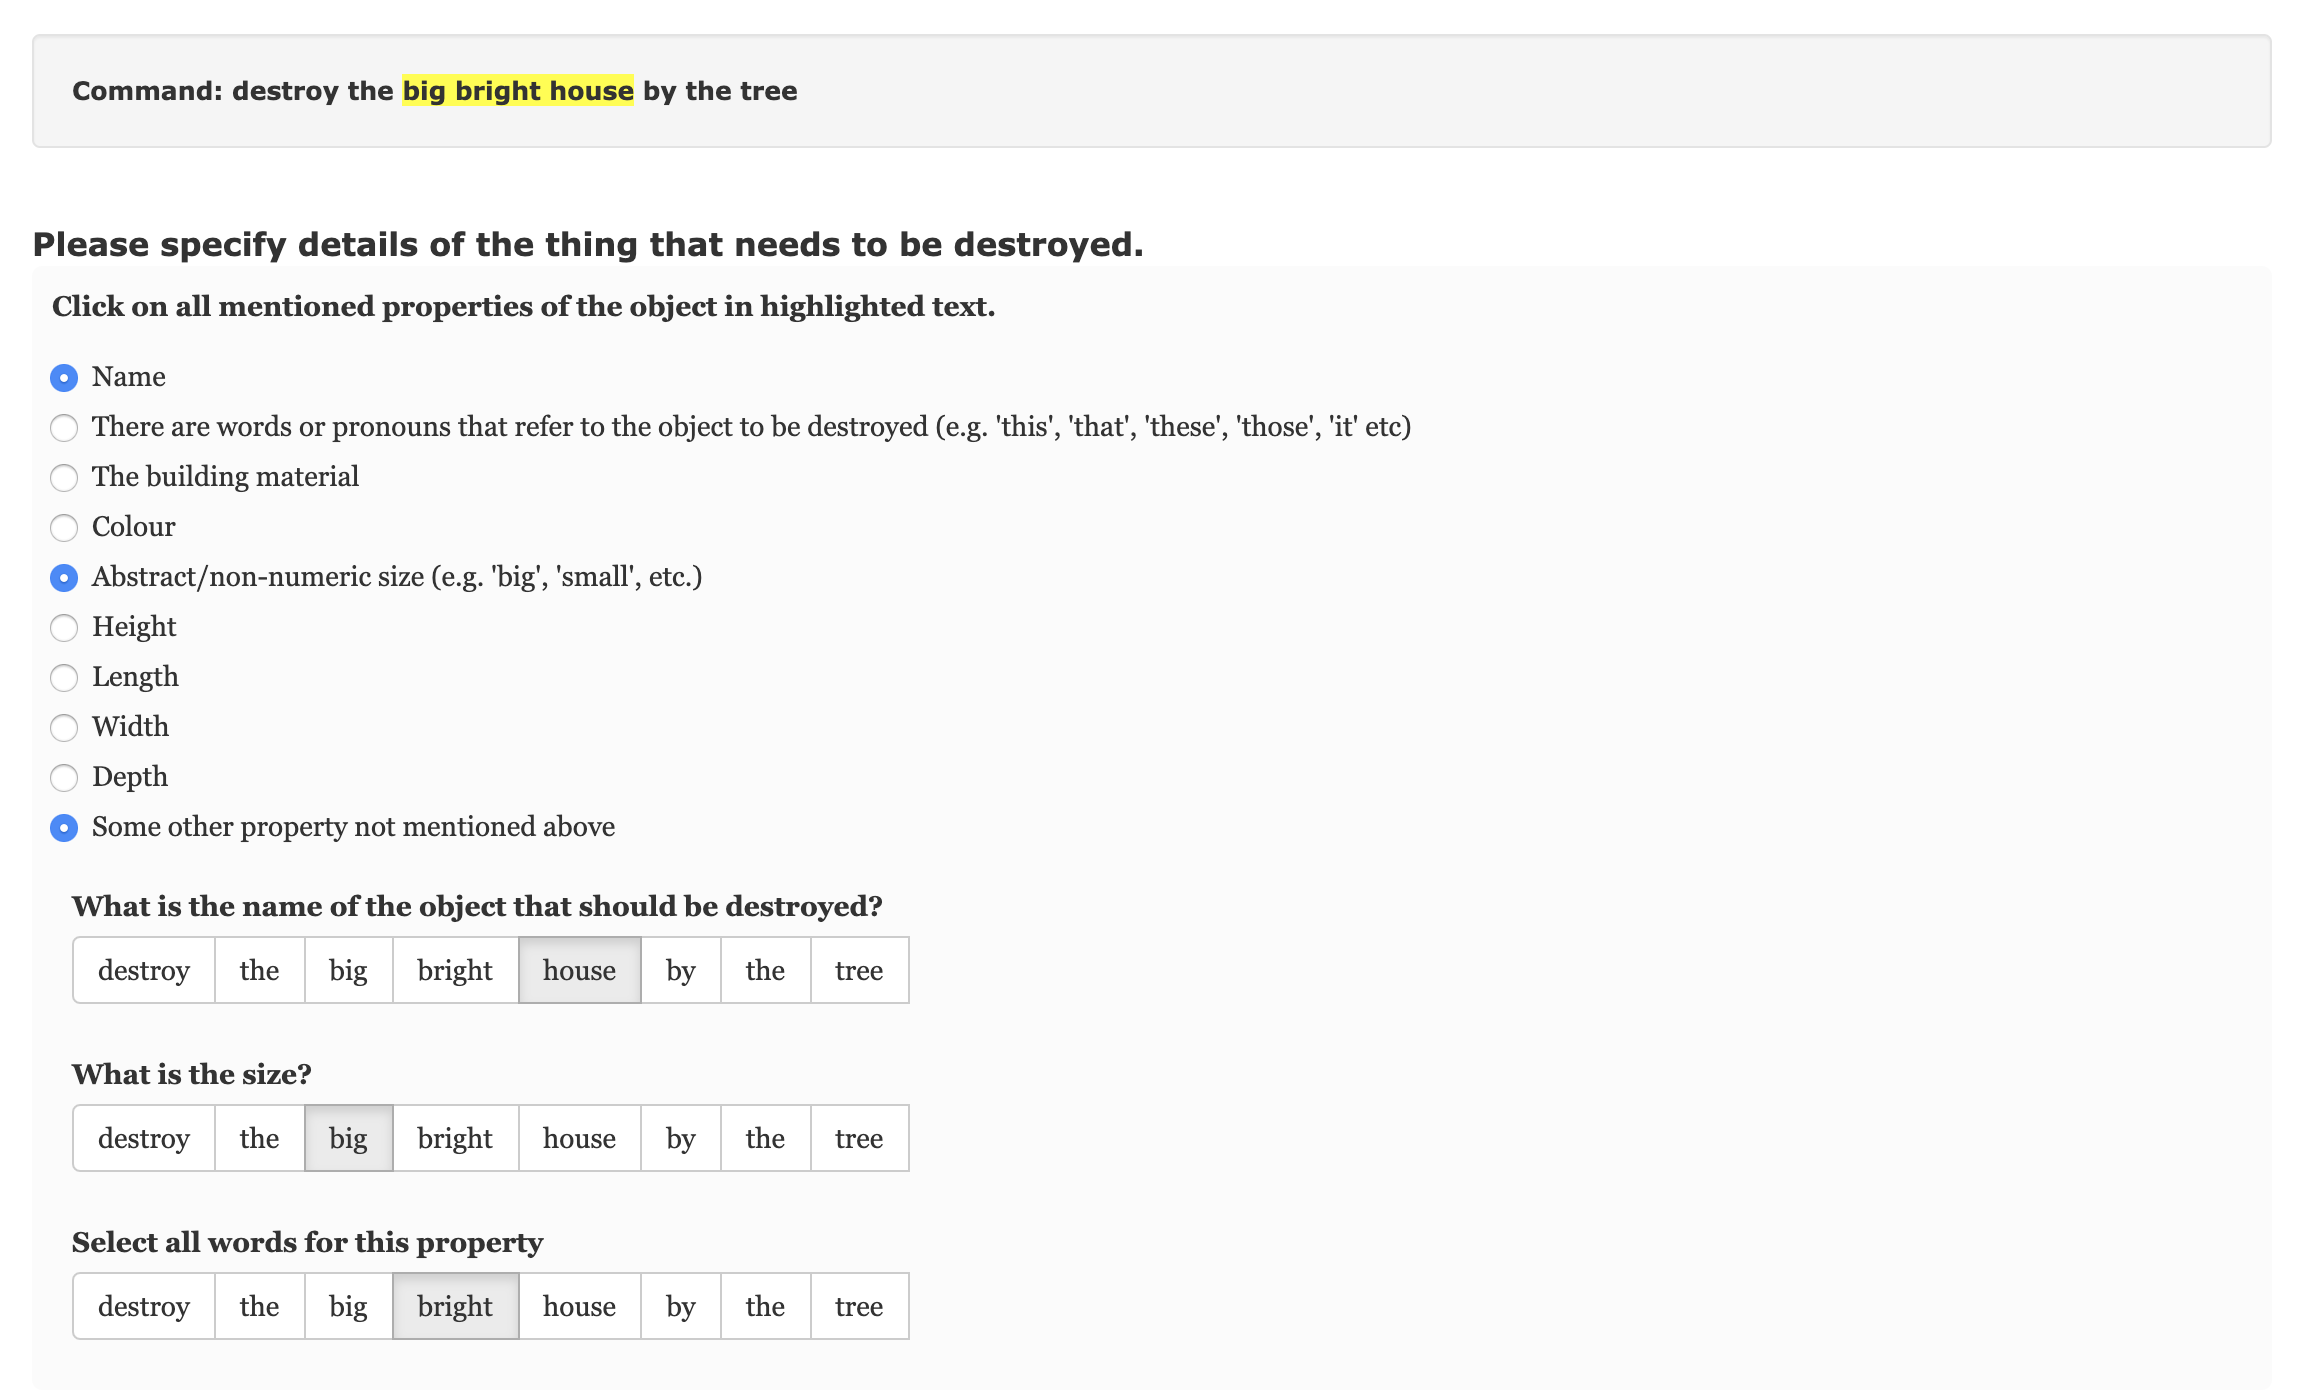
\includegraphics[width=\linewidth, height=6cm, ,keepaspectratio  ]{figures/26.png} 
	 \caption{The step by step screenshot of annotating properties of highlighted words for``reference\_object''  in a ``Destroy'' action.}
	\label{fig:destroy_ref}
\end{figure}

\subsection{Tool for composite commands}
\label{sec:composite}
This tool is meant for ``composite'' commands (commands that include multiple actions) and asks the users to split a command into multiple individual commands. The instruction for this are shown in figure \ref{fig:comp}. Once we get the split, we send out each command to annotation tool described in Section \ref{sec:anntn}
\begin{figure}
	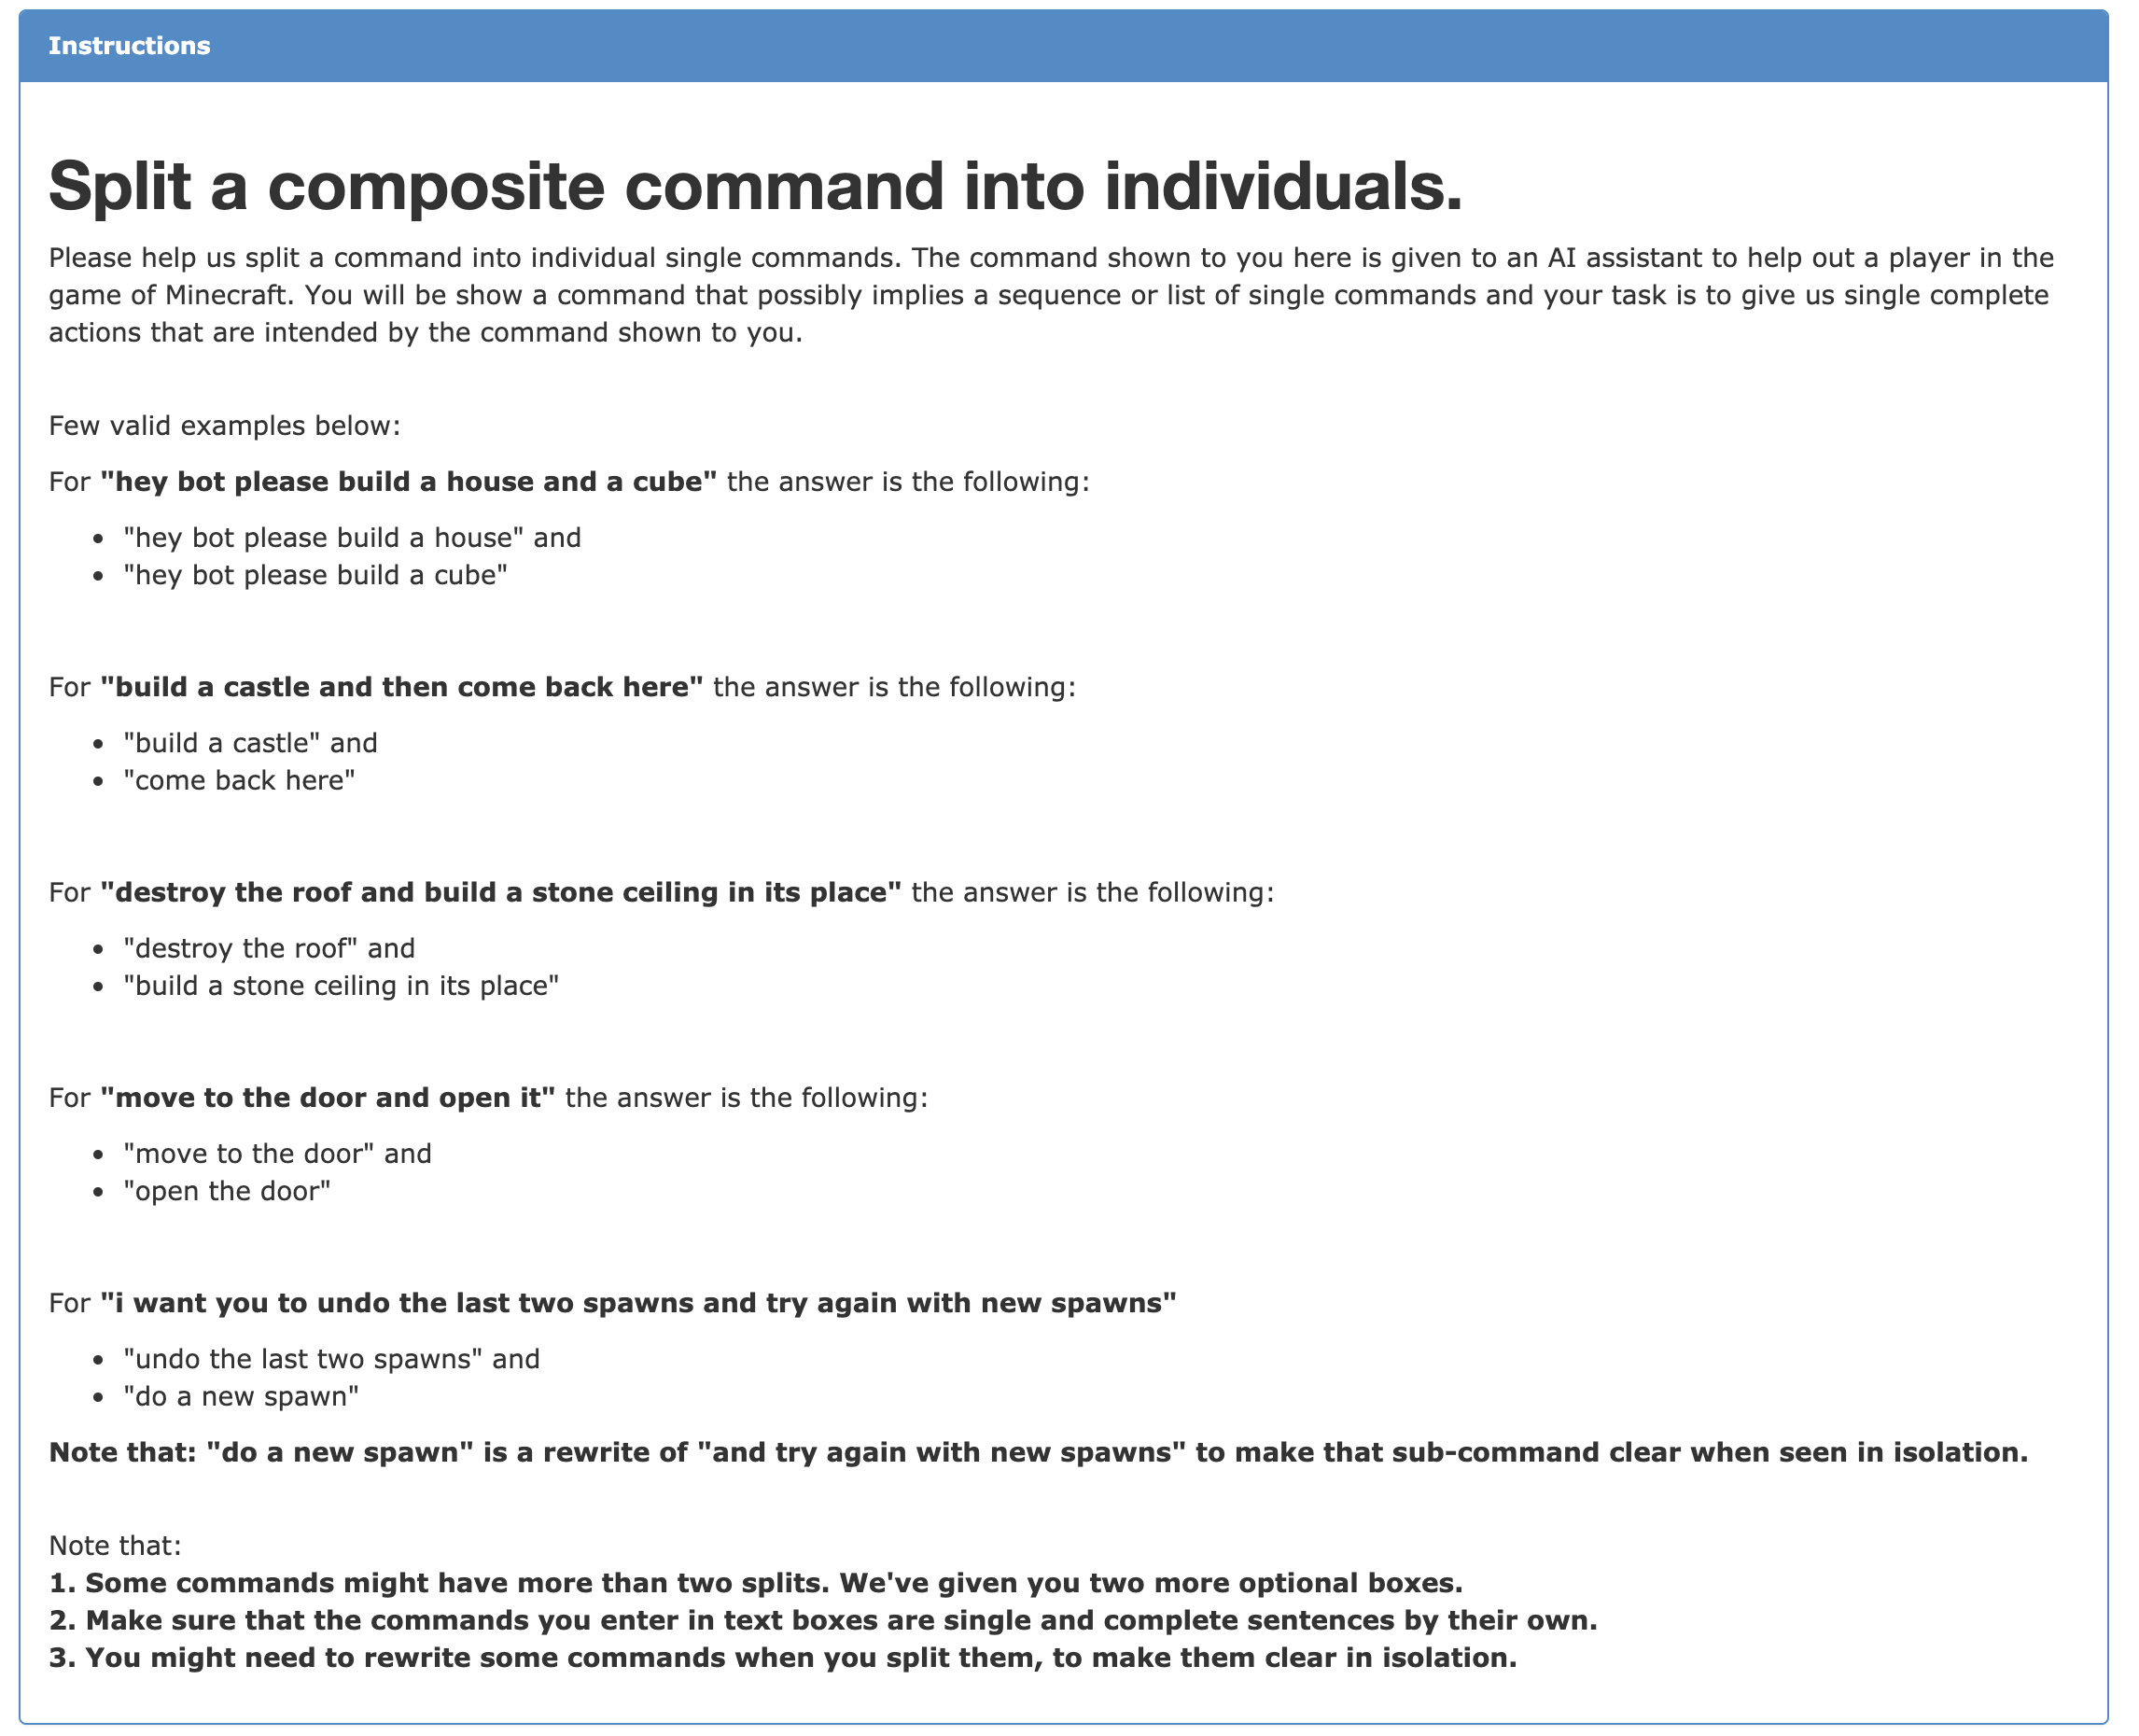
\includegraphics[width=\linewidth ]{figures/composite.png}
	\caption{The task instructions shown to crowd-sourced workers for splitting composite commands}
	\label{fig:comp}
\end{figure}
